% Options for packages loaded elsewhere
\PassOptionsToPackage{unicode}{hyperref}
\PassOptionsToPackage{hyphens}{url}
%
\documentclass[
]{book}
\usepackage{amsmath,amssymb}
\usepackage{iftex}
\ifPDFTeX
  \usepackage[T1]{fontenc}
  \usepackage[utf8]{inputenc}
  \usepackage{textcomp} % provide euro and other symbols
\else % if luatex or xetex
  \usepackage{unicode-math} % this also loads fontspec
  \defaultfontfeatures{Scale=MatchLowercase}
  \defaultfontfeatures[\rmfamily]{Ligatures=TeX,Scale=1}
\fi
\usepackage{lmodern}
\ifPDFTeX\else
  % xetex/luatex font selection
\fi
% Use upquote if available, for straight quotes in verbatim environments
\IfFileExists{upquote.sty}{\usepackage{upquote}}{}
\IfFileExists{microtype.sty}{% use microtype if available
  \usepackage[]{microtype}
  \UseMicrotypeSet[protrusion]{basicmath} % disable protrusion for tt fonts
}{}
\makeatletter
\@ifundefined{KOMAClassName}{% if non-KOMA class
  \IfFileExists{parskip.sty}{%
    \usepackage{parskip}
  }{% else
    \setlength{\parindent}{0pt}
    \setlength{\parskip}{6pt plus 2pt minus 1pt}}
}{% if KOMA class
  \KOMAoptions{parskip=half}}
\makeatother
\usepackage{xcolor}
\usepackage{color}
\usepackage{fancyvrb}
\newcommand{\VerbBar}{|}
\newcommand{\VERB}{\Verb[commandchars=\\\{\}]}
\DefineVerbatimEnvironment{Highlighting}{Verbatim}{commandchars=\\\{\}}
% Add ',fontsize=\small' for more characters per line
\usepackage{framed}
\definecolor{shadecolor}{RGB}{248,248,248}
\newenvironment{Shaded}{\begin{snugshade}}{\end{snugshade}}
\newcommand{\AlertTok}[1]{\textcolor[rgb]{0.94,0.16,0.16}{#1}}
\newcommand{\AnnotationTok}[1]{\textcolor[rgb]{0.56,0.35,0.01}{\textbf{\textit{#1}}}}
\newcommand{\AttributeTok}[1]{\textcolor[rgb]{0.13,0.29,0.53}{#1}}
\newcommand{\BaseNTok}[1]{\textcolor[rgb]{0.00,0.00,0.81}{#1}}
\newcommand{\BuiltInTok}[1]{#1}
\newcommand{\CharTok}[1]{\textcolor[rgb]{0.31,0.60,0.02}{#1}}
\newcommand{\CommentTok}[1]{\textcolor[rgb]{0.56,0.35,0.01}{\textit{#1}}}
\newcommand{\CommentVarTok}[1]{\textcolor[rgb]{0.56,0.35,0.01}{\textbf{\textit{#1}}}}
\newcommand{\ConstantTok}[1]{\textcolor[rgb]{0.56,0.35,0.01}{#1}}
\newcommand{\ControlFlowTok}[1]{\textcolor[rgb]{0.13,0.29,0.53}{\textbf{#1}}}
\newcommand{\DataTypeTok}[1]{\textcolor[rgb]{0.13,0.29,0.53}{#1}}
\newcommand{\DecValTok}[1]{\textcolor[rgb]{0.00,0.00,0.81}{#1}}
\newcommand{\DocumentationTok}[1]{\textcolor[rgb]{0.56,0.35,0.01}{\textbf{\textit{#1}}}}
\newcommand{\ErrorTok}[1]{\textcolor[rgb]{0.64,0.00,0.00}{\textbf{#1}}}
\newcommand{\ExtensionTok}[1]{#1}
\newcommand{\FloatTok}[1]{\textcolor[rgb]{0.00,0.00,0.81}{#1}}
\newcommand{\FunctionTok}[1]{\textcolor[rgb]{0.13,0.29,0.53}{\textbf{#1}}}
\newcommand{\ImportTok}[1]{#1}
\newcommand{\InformationTok}[1]{\textcolor[rgb]{0.56,0.35,0.01}{\textbf{\textit{#1}}}}
\newcommand{\KeywordTok}[1]{\textcolor[rgb]{0.13,0.29,0.53}{\textbf{#1}}}
\newcommand{\NormalTok}[1]{#1}
\newcommand{\OperatorTok}[1]{\textcolor[rgb]{0.81,0.36,0.00}{\textbf{#1}}}
\newcommand{\OtherTok}[1]{\textcolor[rgb]{0.56,0.35,0.01}{#1}}
\newcommand{\PreprocessorTok}[1]{\textcolor[rgb]{0.56,0.35,0.01}{\textit{#1}}}
\newcommand{\RegionMarkerTok}[1]{#1}
\newcommand{\SpecialCharTok}[1]{\textcolor[rgb]{0.81,0.36,0.00}{\textbf{#1}}}
\newcommand{\SpecialStringTok}[1]{\textcolor[rgb]{0.31,0.60,0.02}{#1}}
\newcommand{\StringTok}[1]{\textcolor[rgb]{0.31,0.60,0.02}{#1}}
\newcommand{\VariableTok}[1]{\textcolor[rgb]{0.00,0.00,0.00}{#1}}
\newcommand{\VerbatimStringTok}[1]{\textcolor[rgb]{0.31,0.60,0.02}{#1}}
\newcommand{\WarningTok}[1]{\textcolor[rgb]{0.56,0.35,0.01}{\textbf{\textit{#1}}}}
\usepackage{longtable,booktabs,array}
\usepackage{calc} % for calculating minipage widths
% Correct order of tables after \paragraph or \subparagraph
\usepackage{etoolbox}
\makeatletter
\patchcmd\longtable{\par}{\if@noskipsec\mbox{}\fi\par}{}{}
\makeatother
% Allow footnotes in longtable head/foot
\IfFileExists{footnotehyper.sty}{\usepackage{footnotehyper}}{\usepackage{footnote}}
\makesavenoteenv{longtable}
\usepackage{graphicx}
\makeatletter
\def\maxwidth{\ifdim\Gin@nat@width>\linewidth\linewidth\else\Gin@nat@width\fi}
\def\maxheight{\ifdim\Gin@nat@height>\textheight\textheight\else\Gin@nat@height\fi}
\makeatother
% Scale images if necessary, so that they will not overflow the page
% margins by default, and it is still possible to overwrite the defaults
% using explicit options in \includegraphics[width, height, ...]{}
\setkeys{Gin}{width=\maxwidth,height=\maxheight,keepaspectratio}
% Set default figure placement to htbp
\makeatletter
\def\fps@figure{htbp}
\makeatother
\setlength{\emergencystretch}{3em} % prevent overfull lines
\providecommand{\tightlist}{%
  \setlength{\itemsep}{0pt}\setlength{\parskip}{0pt}}
\setcounter{secnumdepth}{5}
\usepackage{booktabs}
\ifLuaTeX
  \usepackage{selnolig}  % disable illegal ligatures
\fi
\usepackage[]{natbib}
\bibliographystyle{plainnat}
\IfFileExists{bookmark.sty}{\usepackage{bookmark}}{\usepackage{hyperref}}
\IfFileExists{xurl.sty}{\usepackage{xurl}}{} % add URL line breaks if available
\urlstyle{same}
\hypersetup{
  pdftitle={Statistik Deskriptif dengan RStudio},
  pdfauthor={Andri Faisal dan Gatot Soepriyono},
  hidelinks,
  pdfcreator={LaTeX via pandoc}}

\title{Statistik Deskriptif dengan RStudio}
\author{Andri Faisal dan Gatot Soepriyono}
\date{2024-11-08}

\usepackage{amsthm}
\newtheorem{theorem}{Theorem}[chapter]
\newtheorem{lemma}{Lemma}[chapter]
\newtheorem{corollary}{Corollary}[chapter]
\newtheorem{proposition}{Proposition}[chapter]
\newtheorem{conjecture}{Conjecture}[chapter]
\theoremstyle{definition}
\newtheorem{definition}{Definition}[chapter]
\theoremstyle{definition}
\newtheorem{example}{Example}[chapter]
\theoremstyle{definition}
\newtheorem{exercise}{Exercise}[chapter]
\theoremstyle{definition}
\newtheorem{hypothesis}{Hypothesis}[chapter]
\theoremstyle{remark}
\newtheorem*{remark}{Remark}
\newtheorem*{solution}{Solution}
\begin{document}
\maketitle

{
\setcounter{tocdepth}{1}
\tableofcontents
}
\hypertarget{about}{%
\chapter{About}\label{about}}

Buku ini berisi mengenai statistik deskriptif dengan menggunakan perangkat lunak (software) Rstudio. Buku diawali dengan pengertian stataistik deskriptif dan juga membuat struktur data di dalam RStudio. Ada petunjuk pembuatan visualisasi data dan juga menghitung nilai deksriptif dari data.

\hypertarget{usage}{%
\section{Usage}\label{usage}}

Each \textbf{bookdown} chapter is an .Rmd file, and each .Rmd file can contain one (and only one) chapter. A chapter \emph{must} start with a first-level heading: \texttt{\#\ A\ good\ chapter}, and can contain one (and only one) first-level heading.

Use second-level and higher headings within chapters like: \texttt{\#\#\ A\ short\ section} or \texttt{\#\#\#\ An\ even\ shorter\ section}.

The \texttt{index.Rmd} file is required, and is also your first book chapter. It will be the homepage when you render the book.

\hypertarget{render-book}{%
\section{Render book}\label{render-book}}

You can render the HTML version of this example book without changing anything:

\begin{enumerate}
\def\labelenumi{\arabic{enumi}.}
\item
  Find the \textbf{Build} pane in the RStudio IDE, and
\item
  Click on \textbf{Build Book}, then select your output format, or select ``All formats'' if you'd like to use multiple formats from the same book source files.
\end{enumerate}

Or build the book from the R console:

\begin{Shaded}
\begin{Highlighting}[]
\NormalTok{bookdown}\SpecialCharTok{::}\FunctionTok{render\_book}\NormalTok{()}
\end{Highlighting}
\end{Shaded}

To render this example to PDF as a \texttt{bookdown::pdf\_book}, you'll need to install XeLaTeX. You are recommended to install TinyTeX (which includes XeLaTeX): \url{https://yihui.org/tinytex/}.

\hypertarget{preview-book}{%
\section{Preview book}\label{preview-book}}

As you work, you may start a local server to live preview this HTML book. This preview will update as you edit the book when you save individual .Rmd files. You can start the server in a work session by using the RStudio add-in ``Preview book'', or from the R console:

\begin{Shaded}
\begin{Highlighting}[]
\NormalTok{bookdown}\SpecialCharTok{::}\FunctionTok{serve\_book}\NormalTok{()}
\end{Highlighting}
\end{Shaded}

\hypertarget{hello-bookdown}{%
\chapter{Hello bookdown}\label{hello-bookdown}}

All chapters start with a first-level heading followed by your chapter title, like the line above. There should be only one first-level heading (\texttt{\#}) per .Rmd file.

\hypertarget{a-section}{%
\section{A section}\label{a-section}}

All chapter sections start with a second-level (\texttt{\#\#}) or higher heading followed by your section title, like the sections above and below here. You can have as many as you want within a chapter.

\hypertarget{an-unnumbered-section}{%
\subsection*{An unnumbered section}\label{an-unnumbered-section}}
\addcontentsline{toc}{subsection}{An unnumbered section}

Chapters and sections are numbered by default. To un-number a heading, add a \texttt{\{.unnumbered\}} or the shorter \texttt{\{-\}} at the end of the heading, like in this section.

\hypertarget{cross}{%
\chapter{Cross-references}\label{cross}}

Cross-references make it easier for your readers to find and link to elements in your book.

\hypertarget{chapters-and-sub-chapters}{%
\section{Chapters and sub-chapters}\label{chapters-and-sub-chapters}}

There are two steps to cross-reference any heading:

\begin{enumerate}
\def\labelenumi{\arabic{enumi}.}
\tightlist
\item
  Label the heading: \texttt{\#\ Hello\ world\ \{\#nice-label\}}.

  \begin{itemize}
  \tightlist
  \item
    Leave the label off if you like the automated heading generated based on your heading title: for example, \texttt{\#\ Hello\ world} = \texttt{\#\ Hello\ world\ \{\#hello-world\}}.
  \item
    To label an un-numbered heading, use: \texttt{\#\ Hello\ world\ \{-\#nice-label\}} or \texttt{\{\#\ Hello\ world\ .unnumbered\}}.
  \end{itemize}
\item
  Next, reference the labeled heading anywhere in the text using \texttt{\textbackslash{}@ref(nice-label)}; for example, please see Chapter \ref{cross}.

  \begin{itemize}
  \tightlist
  \item
    If you prefer text as the link instead of a numbered reference use: \protect\hyperlink{cross}{any text you want can go here}.
  \end{itemize}
\end{enumerate}

\hypertarget{captioned-figures-and-tables}{%
\section{Captioned figures and tables}\label{captioned-figures-and-tables}}

Figures and tables \emph{with captions} can also be cross-referenced from elsewhere in your book using \texttt{\textbackslash{}@ref(fig:chunk-label)} and \texttt{\textbackslash{}@ref(tab:chunk-label)}, respectively.

See Figure \ref{fig:nice-fig}.

\begin{Shaded}
\begin{Highlighting}[]
\FunctionTok{par}\NormalTok{(}\AttributeTok{mar =} \FunctionTok{c}\NormalTok{(}\DecValTok{4}\NormalTok{, }\DecValTok{4}\NormalTok{, .}\DecValTok{1}\NormalTok{, .}\DecValTok{1}\NormalTok{))}
\FunctionTok{plot}\NormalTok{(pressure, }\AttributeTok{type =} \StringTok{\textquotesingle{}b\textquotesingle{}}\NormalTok{, }\AttributeTok{pch =} \DecValTok{19}\NormalTok{)}
\end{Highlighting}
\end{Shaded}

\begin{figure}

{\centering 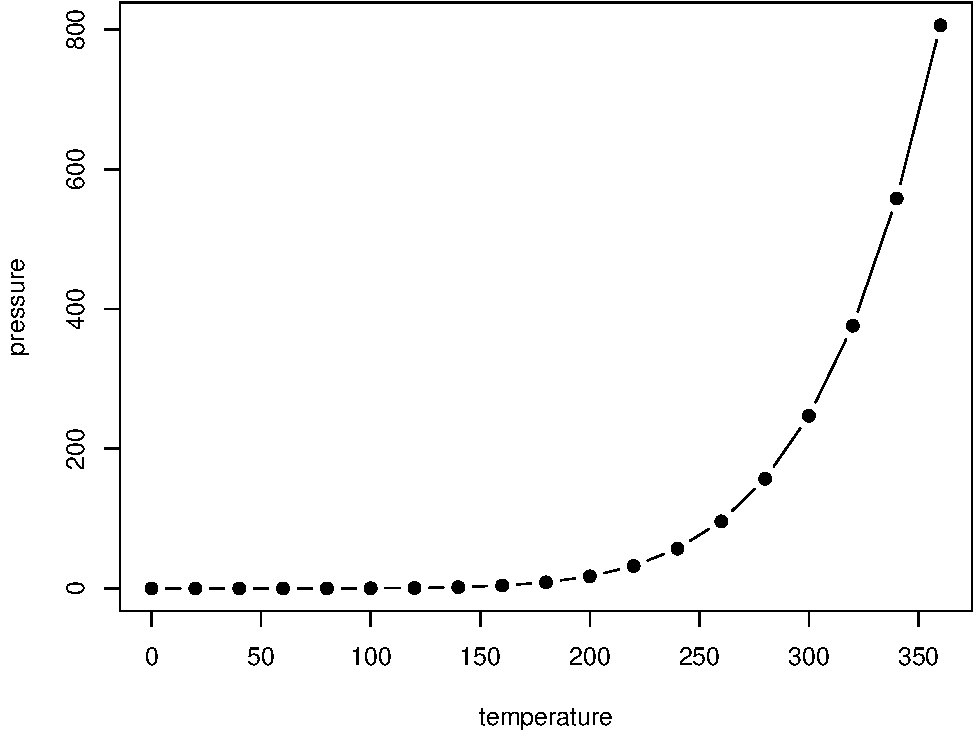
\includegraphics[width=0.8\linewidth]{_main_files/figure-latex/nice-fig-1} 

}

\caption{Here is a nice figure!}\label{fig:nice-fig}
\end{figure}

Don't miss Table \ref{tab:nice-tab}.

\begin{Shaded}
\begin{Highlighting}[]
\NormalTok{knitr}\SpecialCharTok{::}\FunctionTok{kable}\NormalTok{(}
  \FunctionTok{head}\NormalTok{(pressure, }\DecValTok{10}\NormalTok{), }\AttributeTok{caption =} \StringTok{\textquotesingle{}Here is a nice table!\textquotesingle{}}\NormalTok{,}
  \AttributeTok{booktabs =} \ConstantTok{TRUE}
\NormalTok{)}
\end{Highlighting}
\end{Shaded}

\begin{table}

\caption{\label{tab:nice-tab}Here is a nice table!}
\centering
\begin{tabular}[t]{rr}
\toprule
temperature & pressure\\
\midrule
0 & 0.0002\\
20 & 0.0012\\
40 & 0.0060\\
60 & 0.0300\\
80 & 0.0900\\
\addlinespace
100 & 0.2700\\
120 & 0.7500\\
140 & 1.8500\\
160 & 4.2000\\
180 & 8.8000\\
\bottomrule
\end{tabular}
\end{table}

\hypertarget{apa-itu-r}{%
\chapter{Apa itu R}\label{apa-itu-r}}

\hypertarget{perangkat-lunak-r}{%
\section{Perangkat Lunak R}\label{perangkat-lunak-r}}

Sebelum belajar mengenai R tersebut ada baiknya kita mengenal R itu sendiri. R adalah freeware yakni Software yang bebas yang berarti setiap orang dapat memilikinya tanpa harus membayar seperti software lainnya.

R adalah suatu software yang dibangun oleh John Chambers dan rekan-rekannya. Awalnya software ini di bangun di Perusahaan Telekomunikasi Amerika AT \&T (Sekarang namanya Lucent Tekcbogies. Menurut Ros Ilhaka dan Robert Gentlemen yang menemukan perangkat lunak ini. Heuman and Shalabh(2004)

Awalnya R adalah bahasa pemrograman untuk S. Pengembangan bahasa R awalnya untuk statistik dan grafis. Namun kini sudah banyak penggunaan model dari grafik yang ada.

Software R adalah bahasa program dan juga software yang mengelola statistik. Software ini digunakan oleh data miner dan juga statistikawan untuk menghitung data.

R software berbeda dengan Software umunya yang sederhana karena hanya memindahkan file spreadsheet ke dalam softwate statistik begitu selesai tinggal dibklik saja dan dengan mudah untuk hasil dari software tersebut.

R bisa dioperasikan dalam beberapa operating sistem seperti Windows, Mac dan Linux. Tentu saja untuk mendapatkan yang sesuai dengan sistem operasi yang kita miliki maka kita harus terlebih dahulu untuk mendownload terlebih dahulu.

Ketika kita menggunakan R maka kita harus merubah cara yang biasanya tersebut. Awalnya mungkin rumit dalan penggunaan ini karena kita harus mengetik beberapa bahasa. Salah sedikit saja kita tidak akan bisa menghasilkan output sesuai dengan data yang kita miliki.

Selain hasil output berupa tulisan, R juga punya fasilitas untuk membuat grafik yang cantik dan interaktif. Pilihan grafik banyak sekali yang sangat lengkap.

Bagi statistik, R sangat penting karena perangkat lunak ini dapat mengolah data dengan berbagai metode . Adapun beberapa metode yang dapat dilakukan. Dengan R adalah:

\begin{enumerate}
\def\labelenumi{\arabic{enumi}.}
\item
  Statistik Deskriptif .
  Statistik Deskriptif adalah statistik yang sederhana yang menggambarkan data seperti halnya rata-rata, nilai tengah, modus, simpangan baku dan variasi. Pada bagian ini juga bisa untuk mengelola data dalam bentuk grafik seperti grafik scatter, garis, batang, pie, dan lain lain
\item
  Uji Hipotesis
  Dasar ilmu statistik berkaitan dengan uji hipotesis. R dapat mengelola dalam uji hipotesis seperti uji satu sample, uji dua sample berpasangan, dua sample independen.
\item
  Analisis Ragam
  Kalau ada sejumlah data berkelompok yang kita uji apakah sama atau tidak. R bisa untuk melakukan hal itu baik untuk ANOVA maupun Uji Chi Square. baik analaisi Anova satu arah maupun dua arah baik yang tidak berinteraksi dan yang tidak berinteraksi.
\item
  Uji Regresi
  Untuk mengetahui hubungan anatra variabel bebas terhadap variabel tidak bebas. Regresi tersebut dari regresi cross section, data time series dan lain-lain.
\item
  Peramalan
  Pengolahan data juga memerlukan apa yang akan terjadi di masa mendatang. Perkiraan tersebut berasal dari data yang kita peroleh sebelumnya atau data historis. R dapat membantu beberapa emtode permalam time series seperti, AR, MA, ARIMA dan banyak yang lain.
\end{enumerate}

Tentu saja masih banyak metode statistik yang dapat p dikerjakan oleh R. Hal ini karena software R selalu dikembangkan terus menerus oleh para relawan developer dari berbagai penjuru dunia. Misalnya untuk memuat

R mempunyai yang namanya package yang dapat digunakan untuk beberapa analisis. Tidak semua software mempunyai kemampuan yang sama. R yang dasar yang baru di download belum tentu bisa untuk mengerjakan beberapa metode analisis, atau beberapa hal yang terkait dengan metode yang anda pilih.

Terkadang R yang dasar masih membutuhkan package yang dibangun oleh para relawan-relawan programmmer yang membuat membentuk package. Untuk mendapatkan package kita ke website software R untuk mendapatkan package.

Selain untuk ilmu statistik, R juga bisa untuk membantu pemecahan dalam masalah ilmu matematika pada umunya. Software ini bisa menyelesaikan penyeleseian soal Matriks Aljabar Linier. Software ini juga bisa berfungsi sebagai kalkulator biasa (tentu saja kita tidak menggunakan R hanya semata untuk kalkulator yang sangat sederhana sekali)

\hypertarget{apa-itu-statistik-deskriptif}{%
\chapter{Apa Itu Statistik Deskriptif}\label{apa-itu-statistik-deskriptif}}

Buatlah gambaran tentang seorang apakah dia dari mana saja? Apa ia mempunyai nama asal dari mana

Statistik deskriptif hanya untuk pengumpulan dan penyajian data tok. Untuk itu dinamakan statistik deduktif juga statistik deskriptif dia menguraikan atau yang memberikan deskripsi atas data-data tersebut atau menambah keterangan bagi data-data yang ada yang sudah dikumpulkan tersebut..
Suatu statistik deskriptif menggambarkan keadaan fenomena gejala dan situasi yang ada sebelum kita belajar mengemas statistik deskriptif bahwa kita harus mengetahui bahwa ada variabel random yang perlu kita ketahui seperti suhu yang terjadi di suatu daerah, keadaan keuangan beberapa sebuah perusahaan yang terdaftar di bursa efek Indonesia nilai dari biji suatu kebutuhan bahan pangan pendapatan di suatu kabupaten, dan juga kemampuan guru.

Dalam statistik deskriptif kita bisa mendapatkan beberapa contoh dalam buku yang saya baca ini

\begin{enumerate}
\def\labelenumi{\arabic{enumi}.}
\tightlist
\item
  kebanyakan perusahaan yang sudah mulai bangkrut adalah perusahaan yang mempunyai hutang lebih besar daripada asetnya yakni berkisar 50\% lebih banyak daripada asetnya.
  Mahasiswa yang menyelesaikan program sarjana biasanya 90\% tidak terkendala pada semester pertama atau semester kedua.
  Kita harus memperhatikan bahwa ada beberapa data yang sudah kita kumpulkan lalu kalau kita mengikut daripada data yang sudah ada disebut yang kita menguburkan lebih menjadi beberapa data-data tersebut disatukan satu sama lainnya karena mempunyai sifat yang berbeda. Asalnya adalah beberapa data tersebut jika diberikan menjadi berikut
\end{enumerate}

data nominal

Data seperti ini adalah data kualitatif yang sebenarnya menggolongkan dalam beberapa hal karena itu bisa jadi acara ini dan dari kualitatif dengan beberapa kriteria tertentu hingga dimasukkan menjadi data nominal. Apa artinkata nominal?
Misalnya kita memberikan waktu kelahiran seseorang itu dimaksud dengan data nominal karena datanya bisa meningkatkan dan bukan berarti kemudian kita juga akan dikelompokkan beberapa kategori atau badan seperti ini atau mungkin dari agama atau operasinya dari organisasi.

Data ordinat adalah data yang dikelompokkan juga sama halnya dengan data nominal lain hanya dengan nominal pada tahun 197 sudah berdasarkan kategori tertentu yang penilaian itu berdasarkan dari yang terendah terbesar atau sebaliknya. Contoh dari data koordinasi seperti rangking siswa di satu kelas.

Data interval

Perhatikan interval adalah data yang ada diatas dan membagi data tersebut seperti nominal dan ordinal. Maka ada satu ciri khas yang dalam data ordinal yakni penambahan berupa urutan kategori yang seperti itu dengand ata ordinal yaknimamin pembagiannya berdasarkan kisaran yang sama.

Contoh kita membagidata ABCDE dengan angka 12345 maka dari setiap kategori tersebut adalah mempunyai nilai yang berbeda satu dengan yang lainnya

Data Rasio
Data inilah yang mempunyai data yang lengkap dari ketiga data diatas. Memiliki angka 0 absolulut dan mempunyai makna yang empiris . Contoh adalah nilai dari Amir mendapatkan 20
Inilah mempunyai nilai yang sebenarnya dalam bentuk penilaian O itu tidak ada seperti anak yang beroperasi nol . Atau mungkin ada yang tanah niainya nol kecuali ada gak punya tanah

Analisa Statistik deskriptif menggunakan MAtLAb cetakan pertama 2008 Graha Ilmu Deddy Barnabas Lasfeto. oki Dwi Nurhayati ISBN 978-979-736-372-1. Yogyakarta

Statistik Deskriptif. Dodi Wahab dan Andri Nur. 2001. Cetakan pertama dan edisi pertama

Kemudian ada dananya data diakrit yang hanya menempati titik tertentu saja. Maka kita tidak bisa mengatakan. Ada anak sejumlah setengah aja.

Ada data kontinues yang bisa menempati antara data atau titik yang disebut juga berkesinambungan. Pada contoh ini adalah jumlah uang dalam jumlah pecahan hingga koma yang mewakili per sen.

Kalau kita tabulasi maka ada data yang dapat berupa data diskrit dari keempat jenis data diatas yakni bisa nominal, ordinal, interval dan rasio. Hanya data kontinues berlaku pada interval dan rasio saja.

Pada bagian pengumpulan data adalah proses pencatatan atau peristiwa dari karakteristik elemen yang akan menjadi penelitian. Data dikumpulkan dalam tabel dan bias aha baris pertama adalah header. Kemudiannada kolom yang mewakili karakter dan di ssbelah kiri adalah nomor yang menunjukkan angka dari individual yang kita sudah cari. Pada bagian akhir adalah sumber dari data. Sumber dari data adalah skeinder kalau kita membuat data dari lembaga, badan , perusahaan atau peneliti lain. Kalau data itu merupakan pengumpulan kita maka kita bisa menuliskan sumber data primer dan jangan lupa menyebutkan tahunnya.

Pada pengerjaan tabel di rstudio cukup repot tetapi bukan tidak bisa anda bisa langsung membuat tabel atau membuat terlebih dahulu data frame.

Sebelum melangkah jauh mengenai statistik kita berbicara mengenai data terlebih dahulu. ilmu statistik tidak akan kita dapati tanpa data maka kita tidak akan mengerti apa yang namanya statistik tersebut.

Data adalah sesuatu yang penting. Menurut beberapa ahli, data adalah sesuatu. Sesuatu adalah menggambarkan sesuatu mahluk atau benda mati. data ada di mana- mana dari lingkungan yang Sangat besar hingga lingkungan yang kecil.

Dalam diri kita ada data. Saat kita kecil sudah dapatkan nama dari orang tua kita. Itu yang membedakan kita dengan individu yang lainnya. Pihak rumah sakit akan mencatat berat, tinggi bayi, cap kaki bayi bahkan golongan darah. Semua itu akan menjadi data dalan akte kita.

Semakin meningkat manusia akan memiliki banyak sekali data. Mulai dari kartu identitas, dimana ia sekolah, dimana ia bekerja, dimana ia beribadah dan dimana ia bersosialisasi dan dimana yang lainnya. Semuanya akan menjadi data yang dapat berguna bagi dirinya sendiri atau bagi orang lain.

Data bisa jadi berupa reputasi dari orang tersebut jika ia mempunyai suatu kebaikan dan integritas dalam dirinya. Bisa jadi ada yang berdusta atau yang terlalu berlebihan namun itu sebenarnya adalah realitas sebuah data.

Mungkin akan ada pertanyaan apakah data bohong. Sebagai benda mati, data tidak bohong dan tidak ada data yang jelek ataupun jahat. Data yang bohong itu bisa diperoleh oleh pengumpulnya yang tidak jujur. Mereka berbohong untuk kepentingan diri ataupun kelompoknya. Data tersebut mungkin sudah lama tersimpan bisa mempengaruhi orang lain.

Bisa jadi kebohongan tersebut karena sumber yang tidak benar. Terkadang sumber yang tidak benar itu terjadi karena permasalahan sepele yakni kemalasan dari sang Narasumber untuk menjawab sampai yang benar-benar bohong karena khawatir akan menjadi konsekuensi dari suatu hal.

Penggunaan data kapan? Sejak zaman dahulu penggunaan data yang seiring dengan adanya manusia di muka bumi. Mereka ingin menghitung berapa banyaknya ternak. Maksudnya adalah agar ternak mereka terjaga. Mereka mengetahui mana yang menjadi ternak mereka dan Manau yang bukan menjadi ternak mereka.

Perhitungan itu berkaitan dengan kewajiban mereka memberi pakan dan juga bagi mereka yang sudah banyak apakah perlu dijual atau dibatasi saja. Semuanya berguna dengan hal itu.

Cerita pertama di Pemerintahan Roma Super power pada masa sebelum Masehi mencatat seluruh warganya yang berada di Roma. Hal it akan berkaitan mengenai penghuni penduduk Roma yang akan membayar pajak. Mereka yang tercatat dalam sejarah melakukan sensus pada penduduknya.

Kini perhitungan sensus di tiap negara dilakukan tentu berdasarkan kemampuan negera tersebut. jika negara yang besar maka dapat menyensus hampir seluruh warganya sebaliknya di negara miskin hal ini sulit sekali karena hal ini berkaitan dengan pendanaan.

Kalau di negeri kita ada yang namanya Badan Pusat Statistik yang menyensus seluruh data warga negara. Pada masa saat ini, BPS lah yang bertugas untuk mengumpulkan data untuk berbagai keperluan negara dan warga negara.

Pemerintah yang bertujuan untuk menyejahterakan masyarakat dan berarti mencukupkan seluruh kebutuhan hidup masyarakat baik aandang, pangan dan papan.

Para ilmuwan juga mempelajari statistik memenuhi untuk mencari ilmu yang selalu berkembang. Apa jadinya jika ilmu tidak ada pembuktian Batang Hari itu hanya sekedar teori teori pajak yang tidak ada semuanya aku alasan dan bukti bukti tersebut

Dengan adanya statistik maka para ilmuwan dapat membuktikan bahwa faktor yang mempengaruhi suatu akibat adalah faktor tertentu. Untuk itulah dengan menggunakan software yang dimiliki oleh R maka akan dapat menemukan factor mana yang berpengaruh terhadap suatu faktor. Jika penggunaan software ini digunakan maka akan dapat menunjang perkembangan ilmu pengetahuan.

Seperti data yang tidak terhitung warna. Kita tidak akan bisa membuat rata-rata warna dari sekumpulan kulit manusia. Oleh karena itu ada beberpa data yang bisa kita kenal sebelum kita bisa mengenal dalam mengelola data-data tersebut.

\begin{enumerate}
\def\labelenumi{\arabic{enumi}.}
\item
  Data Kualitatif adalah data yang menunjukan kualitas dari suatau keadaan tertentu. Bisa jadi data tersebut mengenai warna, rasa, sikap dan lain-lain.
\item
  Data Kuantitatif
  Data yang berupa angka atau menunjukkan satuan bilangan
\item
  Data diskrit
  Data yang tidak bisa dipecah. Data ini hanya bisa menunjukkan pada satu bilangan saja
\item
  Data kontinue data yang bisa ada dalam bilangan interval atau diantara bilangan
\item
  Data Nominal
  Suatu Data yang tidak bisa dihitung tetapi mempunyai nama seperti warna kulit dan rasa
\item
  Data Ordinal
  Data ini mempunyai urutan atau rangking seperti halnya rangking mahasiswa dalam ujian.
  Dalam data nominal kita tidak bisa membuat rata-rata karena hal itu tidak terhitung akan tetapi kita bisa melakukan pengolahan data.
\end{enumerate}

\hypertarget{tipe-dan-struktur-data-r}{%
\chapter{Tipe dan Struktur Data R}\label{tipe-dan-struktur-data-r}}

R berbeda dengan Excel yang menyusun data bagai dengan kolom dan juga harus. Untuk memasukkan data dalam R memang menggunakan dara Excel baik csv dan txt. Ada beberapa macam cara untuk mengolah data dalam R tidak seperti software stataistik lainnya yang hanya menumpulkan data dalam bentuk table dan kemudian mengelolanya.
Terkadang kalau kita menggunakan tipe data dan menggunakan maka kita tidak akan bisa mendaptkan hasilnya yang tidak kita inginkan. Bahkan kalau sebelum belajr R ada baiknya kita mengetahui tipe dan struktur data dari R agar bisa untuk bisa mengetahui untuk belajar lebih banyak lagi mengenai R.

Ada berbagai jenia data namun untuk dasar kita perkenalkan seperti dibawah ini :

\hypertarget{data-frame}{%
\section*{1. Data Frame}\label{data-frame}}
\addcontentsline{toc}{section}{1. Data Frame}

Data frame data frame adalah suatu data yang sering dipakai karena ini adalah kumpulan dari vector yakni data yang sederhana saja yang ditulis dalam bentuk koma.

Data frame seperti halnya kumpulan data saja yang bisa misalnya kita mengumpulkan dari berbagai jenis vector saja dengan karakteristik dengan satu saja atau univariate.Dengan menggabungkan data kita bisa membuat sebuah data frame. Untuk membuat maka kita bisa untuk menjadi data frame.

Data frame setidaknya ada data yang biasa yang memuat data cross section. Dan juga data time series (dijelaskan dalam data). Ada juga data gabungan campuran data dari vector. Jika kita mau untuk membandingkan vector yang satu dengan vector yang lain bisa kita gabungkan

Dari sini sesuai dengan buku ini kita bisa mengelola dalam bentuk analisis lainnya baik descriptive dan analisis inferensial. Dalam buku ini kita akan membutuhkan data frame untuk time series dan analisis regresi
Contoh Membuat data frame dengan gabungan vector. Contoh di sini membuat vector yang terdiri dari id, saving, dan juga income : untuk id saya memilih huruf dari huruf keempat hingga huruf ke sepuluh

\begin{Shaded}
\begin{Highlighting}[]
\NormalTok{id}\OtherTok{\textless{}{-}}\NormalTok{(letters[}\DecValTok{4}\SpecialCharTok{:}\DecValTok{10}\NormalTok{])}
\NormalTok{id}
\end{Highlighting}
\end{Shaded}

\begin{verbatim}
## [1] "d" "e" "f" "g" "h" "i" "j"
\end{verbatim}

\begin{Shaded}
\begin{Highlighting}[]
\NormalTok{saving}\OtherTok{\textless{}{-}}\FunctionTok{c}\NormalTok{(}\DecValTok{100}\NormalTok{,}\DecValTok{200}\NormalTok{,}\DecValTok{150}\NormalTok{,}\DecValTok{130}\NormalTok{,}\DecValTok{120}\NormalTok{,}\DecValTok{200}\NormalTok{,}\DecValTok{250}\NormalTok{)}
\NormalTok{income}\OtherTok{\textless{}{-}}\FunctionTok{c}\NormalTok{(}\DecValTok{1000}\NormalTok{,}\DecValTok{1200}\NormalTok{,}\DecValTok{1300}\NormalTok{,}\DecValTok{1100}\NormalTok{,}\DecValTok{1500}\NormalTok{,}\DecValTok{1250}\NormalTok{,}\DecValTok{1150}\NormalTok{)}
\CommentTok{\#Setelah selesai, saya akan }
\NormalTok{datcoba}\OtherTok{\textless{}{-}}\FunctionTok{data.frame}\NormalTok{(id,saving,income)}
\end{Highlighting}
\end{Shaded}

Jangan khawatir saya akan tambahkan sehingga saya akan mendapatkan data seperti dibawah ini.

Kita bisa mengelola dari membuat tabel dan grafik yang tidak bisa digunakan oleh data yang lain.
Data frame dapat langsung di copy dari data file excel yang berupa ext csv atau txt (caranya akan diterangkan selanjutnya).

\hypertarget{vector-atomic}{%
\section*{2. Vector Atomic}\label{vector-atomic}}
\addcontentsline{toc}{section}{2. Vector Atomic}

Sesuai dengan namanya vector adalah sekumpulan data yang terdiri dari beberapa elemen. Untuk mmebuat vector tidak sulit hanya memberi nama vector bisa berupa sebuah kata, huruf dan campuran huruf angka. Jangan menggunakan tanda spasi atau tanda baca yang lainnya seperti @,\#,\$, dan lain-lain yang akan menyebabkan perintah tersendiri.
Vector ini untuk digunakan bagi pengolahan data univariate atau data yang tunggal. Vector dapat diterapkan untuk membuat grafik. Untuk membuat data seperti ini kita membuat nama data dn Menyusun dari isi data. Cara ini untuk data yang tidak terlalu banyak kalau sudah terlalu banyak maka cara copy lebih baik disamping lebih sederhana dan kita dapat menyimpan datanya ke dalam file lain yakni excel.
Untuk membuat Vector kita bisa melalukan penulisan
Nama file\textless-c(data,data,data..)
Data bisa berupa angak atau numeris jika kita ingin atau menggunakan data kuantitatif maka kita bisa harus membuat tanda kutip.

\begin{Shaded}
\begin{Highlighting}[]
\NormalTok{coba}\OtherTok{\textless{}{-}}\FunctionTok{c}\NormalTok{(}\DecValTok{100}\NormalTok{,}\DecValTok{200}\NormalTok{,}\DecValTok{300}\NormalTok{)}
\NormalTok{coba}
\end{Highlighting}
\end{Shaded}

\begin{verbatim}
## [1] 100 200 300
\end{verbatim}

\begin{Shaded}
\begin{Highlighting}[]
\NormalTok{cobax}\OtherTok{\textless{}{-}}\FunctionTok{c}\NormalTok{(}\StringTok{"Macan"}\NormalTok{,}\StringTok{"Singa"}\NormalTok{,}\StringTok{"Serigala"}\NormalTok{)}
\NormalTok{cobax}
\end{Highlighting}
\end{Shaded}

\begin{verbatim}
## [1] "Macan"    "Singa"    "Serigala"
\end{verbatim}

R juga dapat membantu kita untuk menambah data yang sudah kita buat seperti fungsi

Typeof(namavektor) -- fungsi ini untuk menunjukkan tipe data dari vektor

length(namavektor) -- fungsi ini untuk menunjukkan berapa banyak data

Class(namavektor) -- fungsi ini untuk mengetahui jenis data

str(namavektor) -- fungsi ini adalah untuk mengetahui jenis struktur data yang sudah kita buat

\begin{Shaded}
\begin{Highlighting}[]
\FunctionTok{typeof}\NormalTok{(coba)}
\end{Highlighting}
\end{Shaded}

\begin{verbatim}
## [1] "double"
\end{verbatim}

\begin{Shaded}
\begin{Highlighting}[]
\FunctionTok{length}\NormalTok{(coba)}
\end{Highlighting}
\end{Shaded}

\begin{verbatim}
## [1] 3
\end{verbatim}

\begin{Shaded}
\begin{Highlighting}[]
\FunctionTok{class}\NormalTok{(coba)}
\end{Highlighting}
\end{Shaded}

\begin{verbatim}
## [1] "numeric"
\end{verbatim}

\begin{Shaded}
\begin{Highlighting}[]
\FunctionTok{str}\NormalTok{(coba)}
\end{Highlighting}
\end{Shaded}

\begin{verbatim}
##  num [1:3] 100 200 300
\end{verbatim}

\begin{Shaded}
\begin{Highlighting}[]
\CommentTok{\#Untuk menamabah data, kita bisa masukkan data seperti ini }
\NormalTok{coba}\OtherTok{\textless{}{-}}\FunctionTok{c}\NormalTok{(coba,}\DecValTok{400}\NormalTok{)}
\NormalTok{coba}
\end{Highlighting}
\end{Shaded}

\begin{verbatim}
## [1] 100 200 300 400
\end{verbatim}

\begin{Shaded}
\begin{Highlighting}[]
\CommentTok{\#Jika hendak menampilkan data berturut kita bisa membuat seperti ini }
\NormalTok{seri}\OtherTok{\textless{}{-}}\NormalTok{(}\DecValTok{1}\SpecialCharTok{:}\DecValTok{7}\NormalTok{)}
\NormalTok{seri}
\end{Highlighting}
\end{Shaded}

\begin{verbatim}
## [1] 1 2 3 4 5 6 7
\end{verbatim}

Data coba sudah ditambahkan 400, dan kalau untuk data non numerik kita bisa lakukan seperti dibawah ini. Perhatikan Ketika kita memanggil vector coba angka 400 sudah masuk ke dalamnya dan vector sebelumnya yang mmeuta tiga anggota saja sudah terhapus

\begin{Shaded}
\begin{Highlighting}[]
\NormalTok{cobax}\OtherTok{\textless{}{-}}\FunctionTok{c}\NormalTok{(cobax,}\StringTok{"Macan Tutul"}\NormalTok{)}
\NormalTok{cobax}
\end{Highlighting}
\end{Shaded}

\begin{verbatim}
## [1] "Macan"       "Singa"       "Serigala"    "Macan Tutul"
\end{verbatim}

\hypertarget{matrix}{%
\section*{3. Matrix}\label{matrix}}
\addcontentsline{toc}{section}{3. Matrix}

Matrix adalah sekumpulan angka yang menempati dalam dua dimensi yakni baik dimensi kolom maupun dimensi baris. Dimensi kolom adalah dimensi yang kebawah sedangkan dimensi baris yang mendatar.
Matrix ini adalah hal yang paling penting dalam pelajaran matematika pada umumnya dan aljebar linear pada khususnya. Tentu untuk pada pengolahan data yang lain bentuk data seperti ini juga digunakan\textgreater{}
Untuk membuat Matrix kita bisa lakukan seperti ini
Namamatrix\textless-matrixc(data,nrow=n,ncol=n)
Dalam contoh matriks n dengan dimensi 3x3 dengan isi angka 1 s.d 9

\begin{Shaded}
\begin{Highlighting}[]
\NormalTok{n}\OtherTok{\textless{}{-}}\FunctionTok{matrix}\NormalTok{(}\DecValTok{1}\SpecialCharTok{:}\DecValTok{9}\NormalTok{,}\AttributeTok{nrow=}\DecValTok{3}\NormalTok{,}\AttributeTok{ncol=}\DecValTok{3}\NormalTok{)}
\NormalTok{n}
\end{Highlighting}
\end{Shaded}

\begin{verbatim}
##      [,1] [,2] [,3]
## [1,]    1    4    7
## [2,]    2    5    8
## [3,]    3    6    9
\end{verbatim}

\hypertarget{list}{%
\section*{4. List}\label{list}}
\addcontentsline{toc}{section}{4. List}

Penggunaan List jarang digunakan pada statistic sederhana dan tidak akan digunakan dalam pembahasan buku yang sederhana ini. Namun untuk pengetahuan dan mungkin bagi yang mau belajar. List adlah sekumpulan data yang beragam tipe data bik itu vector, matrix, dan lain-lain
Untuk mmebuat list maka kita bisa menggunakan formula seperti ini
List adalah salah satu bentuk data dalam Rstudio. Dengan ada LIst kita mengelola data. Keuntungan dari menggunakan list ini adalah kita bisa menyimpan dalam data yang berbeda seperti vektor, data frame, model, fungsi, dan lain-lain. Dengan adanya list kita bisa mudah mengakses ke suatu data tersebut.

\begin{Shaded}
\begin{Highlighting}[]
\CommentTok{\# Membuat list sederhana}
\NormalTok{listku }\OtherTok{\textless{}{-}} \FunctionTok{list}\NormalTok{(}
  \AttributeTok{angka =} \DecValTok{47}\NormalTok{,                   }\CommentTok{\# elemen dengan tipe data numerik}
  \AttributeTok{teks =} \StringTok{"Halo, dunia!"}\NormalTok{,        }\CommentTok{\# elemen dengan tipe data karakter}
  \AttributeTok{vektor =} \FunctionTok{c}\NormalTok{(}\DecValTok{3}\NormalTok{, }\DecValTok{1}\NormalTok{, }\DecValTok{2}\NormalTok{, }\DecValTok{4}\NormalTok{),       }\CommentTok{\# elemen dengan tipe data vektor numerik}
  \AttributeTok{matrix =} \FunctionTok{matrix}\NormalTok{(}\DecValTok{1}\SpecialCharTok{:}\DecValTok{4}\NormalTok{, }\DecValTok{2}\NormalTok{, }\DecValTok{2}\NormalTok{),   }\CommentTok{\# elemen dengan tipe data matriks}
  \AttributeTok{data =} \FunctionTok{data.frame}\NormalTok{(}\AttributeTok{A =} \DecValTok{1}\SpecialCharTok{:}\DecValTok{3}\NormalTok{, }\AttributeTok{B =} \FunctionTok{c}\NormalTok{(}\StringTok{"a"}\NormalTok{, }\StringTok{"b"}\NormalTok{, }\StringTok{"c"}\NormalTok{))  }\CommentTok{\# elemen dengan tipe data data frame}
\NormalTok{)}

\CommentTok{\# Menampilkan isi list}
\FunctionTok{print}\NormalTok{(listku)}
\end{Highlighting}
\end{Shaded}

\begin{verbatim}
## $angka
## [1] 47
## 
## $teks
## [1] "Halo, dunia!"
## 
## $vektor
## [1] 3 1 2 4
## 
## $matrix
##      [,1] [,2]
## [1,]    1    3
## [2,]    2    4
## 
## $data
##   A B
## 1 1 a
## 2 2 b
## 3 3 c
\end{verbatim}

\hypertarget{penyajian-data}{%
\chapter{Penyajian Data}\label{penyajian-data}}

\hypertarget{pengantar}{%
\section{Pengantar}\label{pengantar}}

Setelah data kita kumpulkan maka kita bisa melakukan hal untuk menyajikan data karena seperti disebutkan bahwa data itu ada di mana-mana tetapi tidak bisa dibaca oleh ke semua orang karenanya data perlu dibentuk sajikan dalam beberapa bentuk yaitu setidaknya tabel dan grafik. Bentuk penyajian data ini untuk bisa dibaca oleh orang yang berkepentingan untuk membaca data tersebut memang tidak semua data itu adalah bebas kecuali memang data yang harus diungkap kepada publik harus diberikan penjelasan sejelas-jelasnya kepada para orang yang membutuhkan data tersebut.
Tentunya penting sekali seorang untuk menyajikan data agar bisa terbaca itu maka disajikan dalam bentuk yang mudah dibaca dan mudah dimengerti oleh penggunanya tentu saja. Kalau bagi pengguna orang yang berintelektual maka cukup bisa disajikan dalam bentuk yang cukup unik tetapi kalau dibutuhkan kepada masyarakat pada umumnya harus disajikan secara bentuk umum sehingga tidak ada rasa seseorang yang disembunyikan informasi yang penting bagi kepentingan publik ini sesuai dengan undang-undang keterbukaan informasi tersebut. Tentu tidak semua orang bisa menyajikan data dan terkadang dengan bentuk penyajian data yang tidak bisa atau tidak bisa menyajikan data akan memberikan satu interprestasi yang salah di kalangan masyarakat bisa jadi atau penggunaannya usernya dengan penyajian yang salah bisa jadi akan membuat suatu keputusan yang salah juga karena berdasarkan informasi yang salah yang keliru maka akan menghasilkan informasi yang keliru juga

Penyajian data yang paling penting adalah tabel dari tabel bentuknya itu sederhana setelah kita mengumpulkan data tersebut kita akan mengkompilasikan atau mengumpulkan data-data yang sejenis dan dimasukkan dalam kategori tertentu misalnya berapa jumlah siswa yang ada di kampus. itu akan dibagi dalam beberapa kategori misalnya kategori tahun angkatan dari angkatan pertama sampai angkatan ke-4 kemudian juga dibagi lagi menjadi kategori beberapa yakni seperti jurusan ataupun program studi tersebut bisa saja manajemen, akuntansi, ekonomi, komunikasi, administrasi bisnis ilmu politik dan ilmu Hukum
Kalau kita membaca tabel maka kita harus dengan melihat hati-hati itu semuanya harus perkaranya adalah hati-hati karena mengenai masalah data agar tidak terjadi suatu kesalahpahaman dalam pengambilan keputusan dengan membaca tabel ini sebenarnya kita harus meniti satu demi satu kategori sehingga kita dapat menyimpulkan apa yang kategori yang mempunyai paling banyak misalnya kita di suatu daerah apa suatu produk yang paling laku di daerah tersebut maka mau tidak mau kita harus melihat seluruh daerah yang mempunyai kategori ini nggak mungkin tidak mudah seperti ini ya terlebih kalau jumlah tabelnya itu banyak sekali nah karenanya seorang itu harus bisa mampu menjanjikan data dengan bentuk yang bisa diterima oleh pengguna tentu kalau penggunanya akademisi ya berbeda dengan pengguna pada masyarakat harus disesuaikan dengan membuat penyajian data yang bisa digunakan oleh pengguna (user).
Dalam membuat tabel kita akan melihat bahwa pada bagian-bagian pertama yang akan harus dipenuhi setidaknya oleh pembuat tabel itu bukan hanya sebuah kotak-kota yang berisi kategori tetapi dengan angka tetapi juga lebih dahulu ada bagian bisa jadi kalau orang yang sudah memahami maka halnitu tidak menjadi masalah sebab ia mampu untuk menerjemahkan dan menginterpretasikan apa yang ada dalam tabel tersebut.

Tentu ada beberapa hal atau bentuk penyajian data yang biasa digunakan yaitu pertama grafis ini suatu gambar yang bisa bentuk garis kotak-kotak tersebut dengan adanya grafik ini seseorang bisa langsung membaca data dengan baik tentu untuk bentuknya tidak semua bisa seperti grafik kotak atau box plot itu bagi saya bagi penulis itu sangat susah untuk diterjemahkan karena ada satu kotak tapi ada garis-garis tertentu yang mungkin tidak akan bisa dibaca oleh orang yang terpajak sekalipun tetapi dengan nanti dikatakan kalau grafik yang berbentuk sederhana seperti grafik garis batang atau lingkaran itu hampir semua orang dan kebanyakan orang yang sudah bersekolah sudah bisa membaca maksud dari data-data tersebut. Harga baru tidak dipungkiri bahwa dengan adanya grafik membuat tulisan menarik dan dia seperti merangkum dari semua deskripsi data-data yang sudah diolah ke dalam bentuk yang sangat sederhana sekali bisa jadi dari 5 tulisan maksudnya 5 halaman tulisan akan bisa tergambarkan lewat satu gambar saja yang sangat sederhana tersebut gitu daripada menggambarkan dalam bentuk tulisan yangbanyak sekali.
Grafik apa yang akan saya pilih dalam penyajian data. Itu bergantung dengan yang menjadi kebutuhan. Dari penyajian data tersebut dan tentu juga akan berpengaruh pada data itu sendiri. Ada
Bebeapa daata yang tidak cocok dengan jenis grafik. Misalnya grafik garis tidak cocok diterapkan pada data cross section penjualan makanan di sebuah toko dalam waktu satau periode (bisa tahun, bulan dan hari)
Jenis grafik banyak sekali. Apalagi kalau banyak sekali perangkat lunak yang dapat untuk membuat suatu grafik yang bagus sekali namun pada dasarnya grafik ini terbagi dalam beberapa model seperti :

\hypertarget{grafik-garis}{%
\section{Grafik Garis}\label{grafik-garis}}

Grafik ini adalah grafik yang paling sederhana yang dapat untuk menggambarkan suatu perkembangan suatu data. Yang ada. Dalam grafik garis kita akan melihat trend yang meningkat karena suatu kenaikan atau data yang meningkat perlahan-lahan ataupun bisa peningkatan tersebut melonjak begitu tajam karena daya yang meningkat aecara tajam.

\begin{Shaded}
\begin{Highlighting}[]
\NormalTok{roket}\OtherTok{=}\FunctionTok{c}\NormalTok{(}\DecValTok{2}\NormalTok{,}\DecValTok{3}\NormalTok{,}\DecValTok{5}\NormalTok{,}\DecValTok{6}\NormalTok{,}\DecValTok{7}\NormalTok{,}\DecValTok{10}\NormalTok{,}\DecValTok{13}\NormalTok{,}\DecValTok{3}\NormalTok{,}\DecValTok{4}\NormalTok{)}
\FunctionTok{plot}\NormalTok{(roket)}
\end{Highlighting}
\end{Shaded}

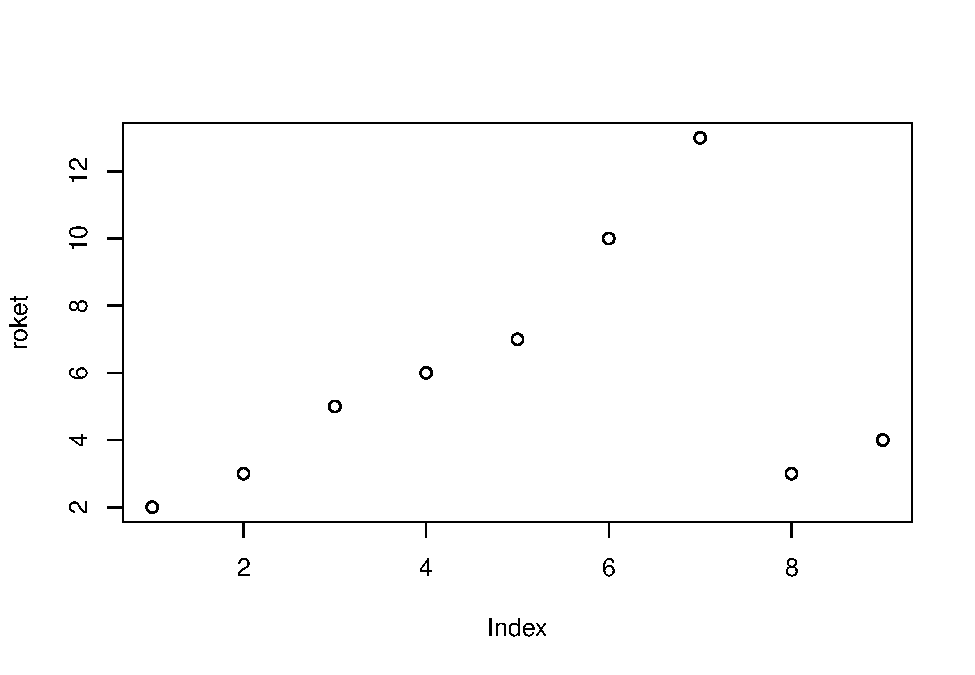
\includegraphics{_main_files/figure-latex/unnamed-chunk-10-1.pdf}

\begin{Shaded}
\begin{Highlighting}[]
\CommentTok{\#jika mau merubah gaya grafik}
\FunctionTok{plot}\NormalTok{(roket,}\AttributeTok{type=}\StringTok{"o"}\NormalTok{,}\AttributeTok{col=}\StringTok{"blue"}\NormalTok{)}

\FunctionTok{title}\NormalTok{(}\AttributeTok{main=}\StringTok{"Jumlah Roket Jatuh"}\NormalTok{,}\AttributeTok{col.main=}\StringTok{"red"}\NormalTok{,}\AttributeTok{font.main=}\DecValTok{4}\NormalTok{)}
\end{Highlighting}
\end{Shaded}

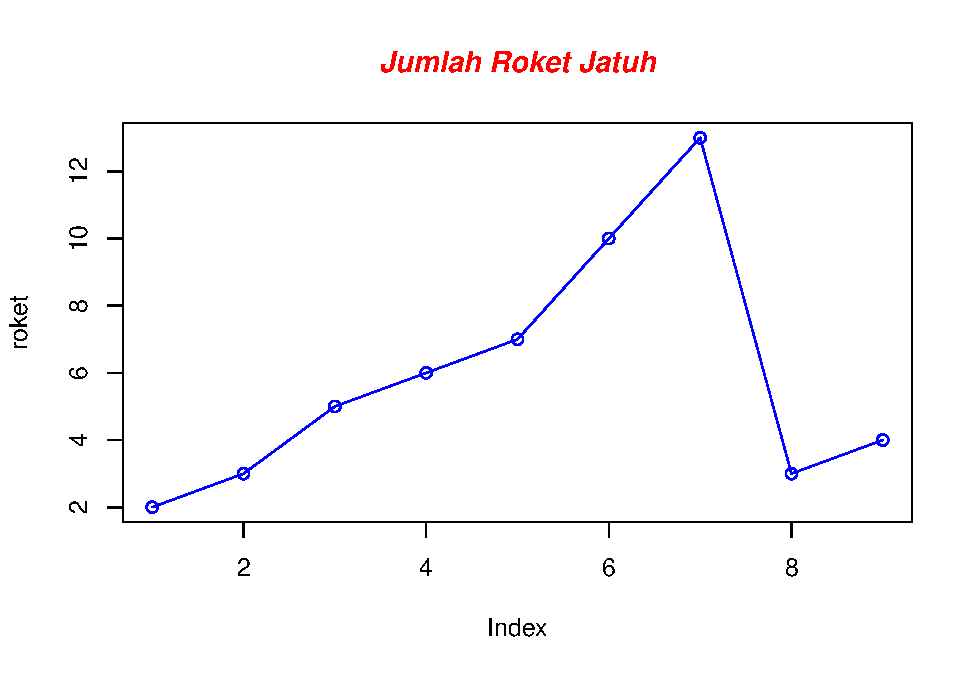
\includegraphics{_main_files/figure-latex/unnamed-chunk-10-2.pdf}

Untuk grafik garis maka yang paling sesuai dengan karakteristik data adalah data time series. Bisa juga data panel yang menunjukka. . apakah kalau data cross section bisa diubah. Maslaah mengubah tidak sulit karena hal tersebut dapat diubah dengan cara memasukkan nilai dan grafik
Analisis grafik untuk mengidentifikasi pola, tren, atau perubahan seiring waktu . Visualisasi memberikan interprestasi dari peningkatan sesuatu data atau penurunan.

\hypertarget{box-plot}{%
\section{Box Plot}\label{box-plot}}

Box Plot adalah Plot atau grafik dalam bentuk kotak atau box. Penampilannya seperti kotak mengambang yang ada bagian tengahnya tersebut.
Untuk mengenali grafik ini maka ada bagian seperti box yang dibagi dua dan juga ada seperti tali di bagian tengah yang disebut juga whiskers.
Bagi Penulis Box Plot cukup merepotkan bagi penulis dan penulis berkeyakinan bahkan mahasiswa kebanyakan tidak dapat mebaca plot tersebut karena memang jarang digunakan apalagi kalau orang umum. Bentuknya kurang umum dibandingan grafik garis, batang, lingkaran maupun gamvar , Sedangkan grafik di sana adalah termausk grafik yang mudah dibca dengan orang yang awam.
KIta melihat kota sebagai representasi dari nilai Kuartil 3 sampain nilai Kuartil satu . Khusus Box plot ini untuk mencari bentuk dari sekumpulan data tersebut. Sekumpulan data atau satu set adalah biasanya yang dijadikan sample . ini digunakan untuk mendeteksi outlier yang biasanya cukup merepotkan adalah data yang berbeda dengan kebanyakan atau juga data ekstrim yang ada dalam sekumpulan data. data outlier adalah data yang ada dalam sekumpulan namun mempunyai nilai yang jauh berbeda dalam rentangan Kuartil satu Maupun kuartil 3 sedangkan nilai ekstrim adalah nilai yang sudah sangat jauh beda. Ini penting karena ada memang data yang dipilih-pilih unuk kesesuaian kegunaan data.
Untuk mendeteksi outlier kita melihat adanya whisker di atas ataupun dibawah box tersebut. kalau ada nlai whisker yang panjang sekalai melebih tiga kali lebar kotak maka itu mengindikasikan adanya suatu nilai ekstrim.

\begin{Shaded}
\begin{Highlighting}[]
\CommentTok{\# Menggunakan data bawaan mtcars}
\FunctionTok{data}\NormalTok{(mtcars)}

\CommentTok{\# Membuat box plot untuk menunjukkan distribusi konsumsi bahan bakar (mpg) berdasarkan jumlah silinder (cyl)}
\FunctionTok{boxplot}\NormalTok{(mpg }\SpecialCharTok{\textasciitilde{}}\NormalTok{ cyl, }
        \AttributeTok{data =}\NormalTok{ mtcars, }
        \AttributeTok{main =} \StringTok{"Box Plot Konsumsi Bahan Bakar Berdasarkan Jumlah Silinder"}\NormalTok{,}
        \AttributeTok{xlab =} \StringTok{"Jumlah Silinder"}\NormalTok{,}
        \AttributeTok{ylab =} \StringTok{"Konsumsi Bahan Bakar (mpg)"}\NormalTok{,}
        \AttributeTok{col =} \FunctionTok{c}\NormalTok{(}\StringTok{"lightblue"}\NormalTok{, }\StringTok{"lightgreen"}\NormalTok{, }\StringTok{"salmon"}\NormalTok{),}
        \AttributeTok{border =} \StringTok{"darkblue"}\NormalTok{)}
\end{Highlighting}
\end{Shaded}

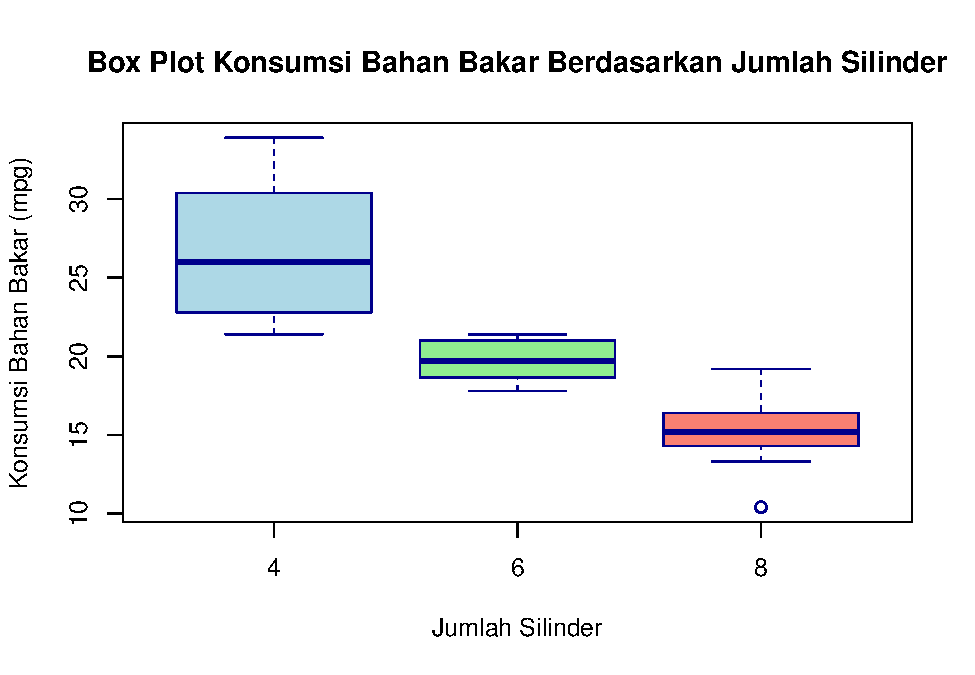
\includegraphics{_main_files/figure-latex/unnamed-chunk-11-1.pdf}

\hypertarget{grafik-batang}{%
\section{Grafik Batang}\label{grafik-batang}}

Sesuai dengan namanya grafik batang adalah berisi batang atau persegi yang dapat untuk mewakili atau representasi data
Pembuatan grafik batang dapat dilakukan manual dengan rangka pembuatan manual kita bisa membuat grafik batang dengan nilai yang sudah ada di dalam tabel tersebut titik memang setiap pembuatan grafik itu tidak akan terlepas dari apa yang namanya tabel kalau kita membuat grafik sebelumnya itu.

\begin{Shaded}
\begin{Highlighting}[]
\CommentTok{\#Membuat Data terlebih dahulu}
\NormalTok{stocktoko }\OtherTok{\textless{}{-}}\FunctionTok{c}\NormalTok{(}\StringTok{"Poly"}\NormalTok{, }\StringTok{"Genius"}\NormalTok{, }\StringTok{"Doma"}\NormalTok{, }\StringTok{"Color"}\NormalTok{, }\StringTok{"Beski"}\NormalTok{)}
\NormalTok{jumlahstock}\OtherTok{\textless{}{-}}\FunctionTok{c}\NormalTok{(}\DecValTok{110}\NormalTok{,}\DecValTok{20}\NormalTok{,}\DecValTok{30}\NormalTok{,}\DecValTok{40}\NormalTok{,}\DecValTok{50}\NormalTok{)}
\CommentTok{\#Membuat data frame }
\NormalTok{stoko}\OtherTok{\textless{}{-}}\FunctionTok{data.frame}\NormalTok{(stocktoko,jumlahstock)}
\CommentTok{\#Membuat Grafik}
\FunctionTok{View}\NormalTok{(stoko)}

\FunctionTok{barplot}\NormalTok{(stoko}\SpecialCharTok{$}\NormalTok{jumlahstock,}\AttributeTok{main=}\StringTok{"stok toko sepeda suka"}\NormalTok{, }\AttributeTok{xlab=}\StringTok{"nama stock"}\NormalTok{, }\AttributeTok{ylab=}\StringTok{"jumlahstock"}\NormalTok{,}\AttributeTok{names.arg=}\NormalTok{stoko}\SpecialCharTok{$}\NormalTok{stocktoko)}
\end{Highlighting}
\end{Shaded}

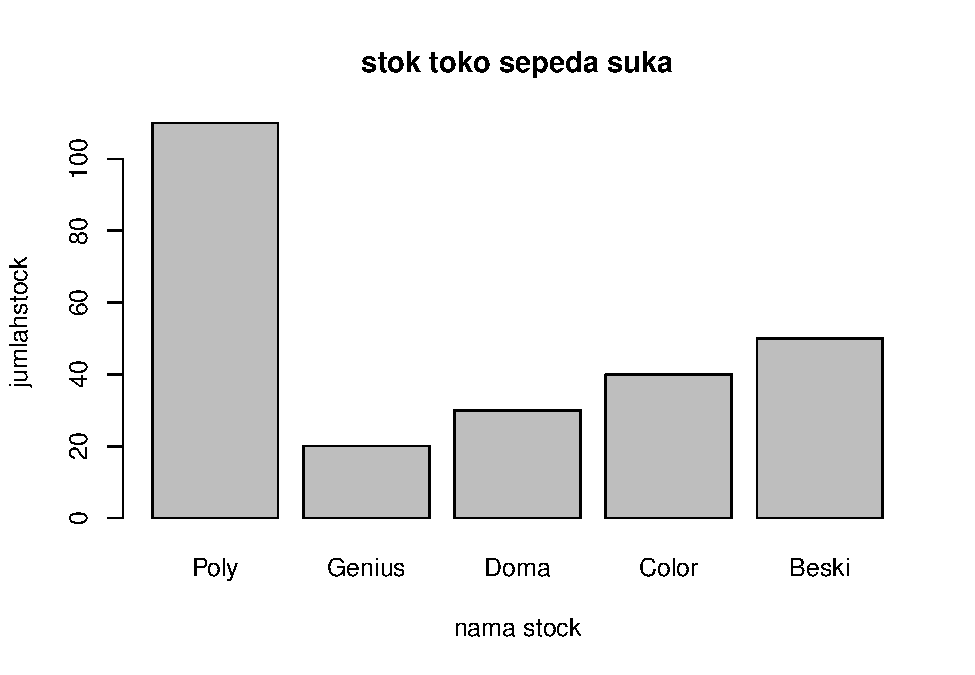
\includegraphics{_main_files/figure-latex/unnamed-chunk-12-1.pdf}

\begin{Shaded}
\begin{Highlighting}[]
\FunctionTok{barplot}\NormalTok{(stoko}\SpecialCharTok{$}\NormalTok{jumlahstock,}\AttributeTok{main=}\StringTok{"stok toko sepeda suka"}\NormalTok{, }\AttributeTok{xlab=}\StringTok{"nama stock"}\NormalTok{, }\AttributeTok{ylab=}\StringTok{"jumlahstock"}\NormalTok{,}\AttributeTok{names.arg=}\NormalTok{stoko}\SpecialCharTok{$}\NormalTok{stocktoko,}\AttributeTok{col=}\FunctionTok{heat.colors}\NormalTok{(}\DecValTok{5}\NormalTok{))}
\end{Highlighting}
\end{Shaded}

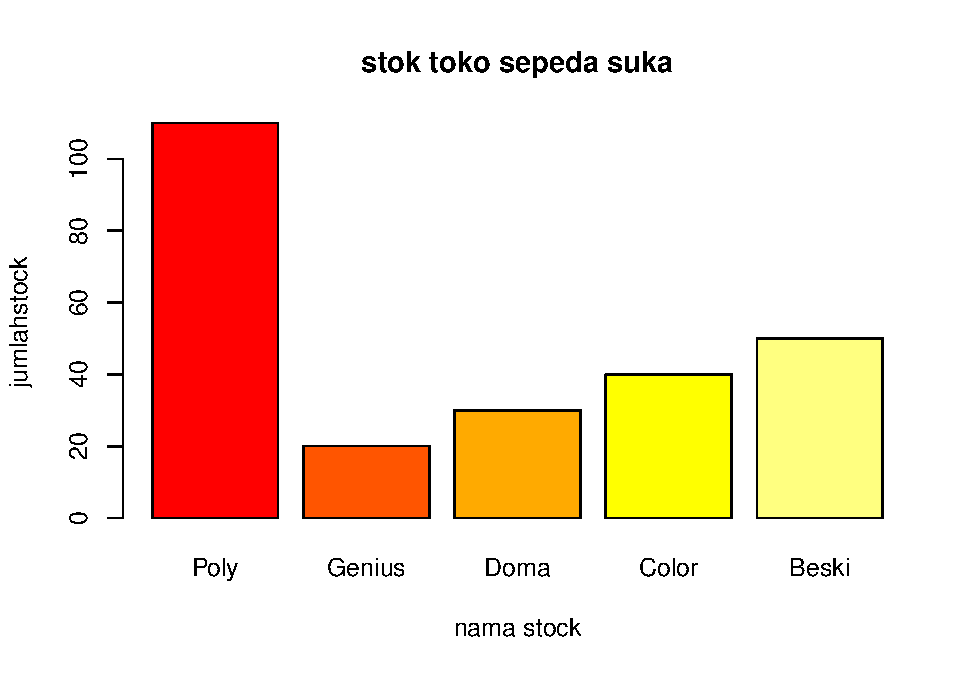
\includegraphics{_main_files/figure-latex/unnamed-chunk-12-2.pdf}

Kita masih memiliki kategori apa saja yang akan kita jadikan limbah tabel misalnya suatu wilayah mempunyai penghasilan sebagai penghasilan kelapa sawit di suatu produksi kita akan membuat batang satu antara kabupaten a yang dihasilkan menjadi poros dari sumbu x atau sumbu horizontal. Kemudian beberapa jumlah dari sumbu y tersebut kalau kita mencontohkan jumlah dari produksi sawit tersebut maka yang tinggi akan diwakili oleh batang yang paling tinggi kita bisa ganti batang kelapa sawit menjadi batang sawit tentu bisa namun judulnya bukan lagi grafik batang grafik gambar dalam grafik batang ada juga grafik yang berbentuk tiga dimensi terdiri atas suatu ruang yang dalam gerakan 3 dimensi atau bahkan 4 dimensi karena itu susah akan seperti waktu atau interaktif hal itu kalau kita hanya ingin menyebabkan maksudnya dalam bentuk seperti buku Harry Potter yang gambarnya atau ilustrasi yang bergerak gitu kalau saya disuruh membuat data tentang data pribadi untuk Anda membuat tahu mau dibuat apa karena kita tidak mempunyai tujuan dalam pengumpulan data tersebut sekali untuk membuat tabel grafik tersebut.
Bagi penulis, box plot cukup untuk mendapatkan penulis berkaitan kalian bahkan tidak ada yang dapat membuat box tersebut lain hanya dengan grafik garis batang atau pie dan sejenisnya merupakan grafik yang mudah dibacakan oleh orang awam sekalipun. Kita melihat kotak itu representasi daripada nilai Q3 sampai Q1 yang dinamakan interkuartil. Khusus buat untuk mencari suatu data tersebut itu mendeteksi suatu dari out layer ataupun data ekstrem yang ada sekumpulan data tersebut data output adalah data yang ada dalam tetapi nilainya berbeda masalah ada yang juga sekali dan ini penting. Karenanya menang data tersebut juga dipilah-pilah untuk kesesuaian dengan kesesuaian.

Box Plot adalah grafik dalam bentuk kotak atau box penampilan seperti kotak yang mengambang diantara tertentu dan bagiannya adalah whisker yang berada di tengah kotak tersebut sedangkan ada nilai Q3 dan Q1 kalau kita akan mencari nilai out player begitu panjang whiskernya itu bisa dia ke bawah ataupun bisa dia juga ke atas.

Membuat garis grafik dapat kita harus menyiapkan data yang akan kita persiapkan untuk grafik kita dengan individu atau juga kategori dan daya adalah data dari periode atau individual kemudian pasangkan nilai sesuai dengan pasangannya baik yang ada di sumbu x maupun juga di garis y kemudian nilai x y dipasangkan maka kita beri titik sehingga sudah dapat anda untuk menyambungkan tiap akan sebagai kita bisa membuat suatu garis apakah grafik garis berlaku untuk beda data

\hypertarget{grafik-pie}{%
\section{Grafik Pie}\label{grafik-pie}}

Grafik PIe dinamakan setelah grafik ini mirip kue Pie yang berbentuk bulat. Gambar grafik pie akan mewakillkan satu kategori saja yang dapat digambarkan kalau ada banyak kategori maka akan sulit saja.
Grafik Pie ini akan memberikan suatau visualisasi yang bagus dengan warna-warna yang menarik dan kontras. Bisa juga dengan membentuk pola seperti arsiran atau pola kalau grafik pie tersebut adalah berwarna hitam dan putih.
Grafik ini akan bagus kalau saja yang idterangkan mempunyai porsi yang hampir mirip seperti mempunyai elemen data hanya empat dan bagian porsi sekitar 25\%. Hanya saja grafik ini akan rumit kalau elemennya lebih dari 10 namun ada yang porsi yang kecil sekalai. misalnya pada saat perhitungan suara pemilu di kpu maka akan terlihat begitu banyak sekali kalau partai-paratai yang berhasil duduk di Senayan alias Gedung MPR dengan partai yang rendah sekali. Ada setidaknya lima partai yang menyempil di bagian tersbeut. seperti grafik lainnya maka akan sulit sekali untuk menebak berapa jumlah proisinya dan mungkin bagi yang kertebatasan dalam penglihatan baik plus ataupun minus maka akan sulit juga untuk melihat seperti ini.
Untuk mmebuatnya secara manual maka kita ahrus menghitung porsi dari data tersebut. Kalau sudah ada data tersedia prosi maka akan dibuat terlebih dahulu bagiannya. LIngkaran atau pie yang ada memang dibagi menurut presentasenya dengan presentase yang besar mendapatkan bagian atau poris yang lebih besar.
Untuk membuat ini kita harus hitung kalau lingkaran tersebut adalah 360 derajat. Untuk membuat suatau lingjaran yang presisi maka kita mmebutuhkan mistar busur yang mungkin sudah lama tidak digunakan (gambar mistar bujur)
misalnya kita menemukan kalau suatu kategori

(kategori dan elemen dijelaskan di awal) bernilai porsi 25 maka kita bisa mengkalikan angka 25\% dengan 360 derajat yang hasilnya 90 derajat. Maka hal itu akan kita hitung sebagai nilai sepermpat yang bisa saja tegak atau mungkin anda memlih yang ada di bagian bawah atau atas selama intu setara dengan 90\% maka itu tidak menjadi masalah.

\begin{Shaded}
\begin{Highlighting}[]
\FunctionTok{pie}\NormalTok{(stoko}\SpecialCharTok{$}\NormalTok{jumlahstock,}\AttributeTok{labels =}\NormalTok{ stoko}\SpecialCharTok{$}\NormalTok{jumlahstock)}
\end{Highlighting}
\end{Shaded}

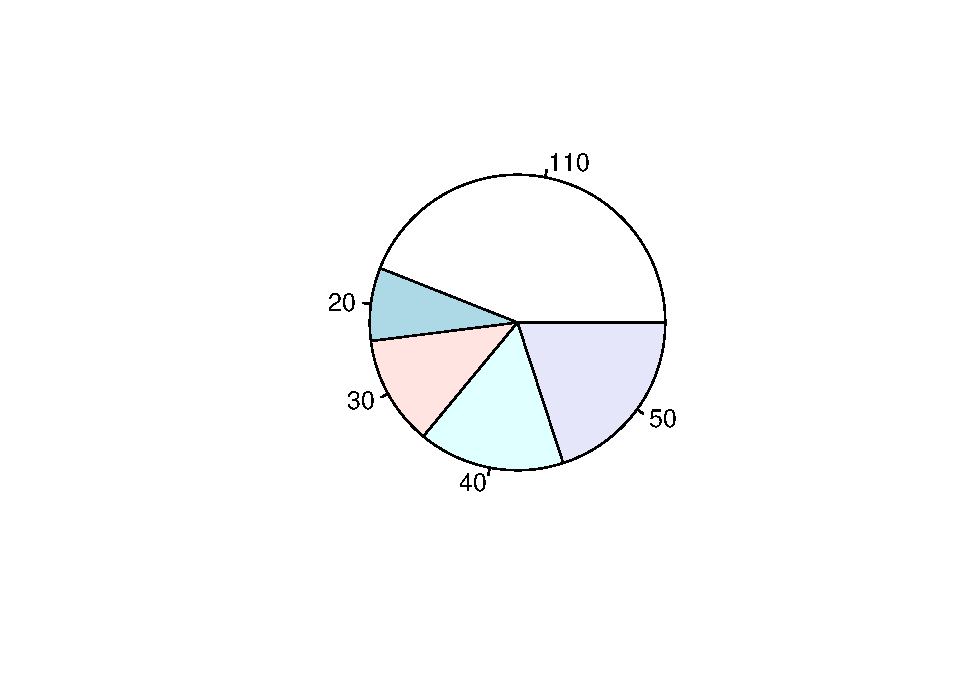
\includegraphics{_main_files/figure-latex/unnamed-chunk-13-1.pdf}

\begin{Shaded}
\begin{Highlighting}[]
\CommentTok{\#Menambahkan judul Grafik}
\FunctionTok{pie}\NormalTok{(stoko}\SpecialCharTok{$}\NormalTok{jumlahstock,}\AttributeTok{labels=}\NormalTok{stoko}\SpecialCharTok{$}\NormalTok{jumlahstock, }\AttributeTok{main=}\StringTok{"Stok Toko Sepeda Suka"}\NormalTok{,}\AttributeTok{col=}\FunctionTok{colors}\NormalTok{(}\DecValTok{5}\NormalTok{))}
\CommentTok{\#Menambahkan Legenda}
\FunctionTok{legend}\NormalTok{(}\StringTok{"topright"}\NormalTok{,}\FunctionTok{c}\NormalTok{(}\StringTok{"Poly"}\NormalTok{,}\StringTok{"Genius"}\NormalTok{,}\StringTok{"Doma"}\NormalTok{,}\StringTok{"Color"}\NormalTok{,}\StringTok{"Beski"}\NormalTok{),}\AttributeTok{cex=}\FloatTok{0.7}\NormalTok{,}\AttributeTok{fill=}\FunctionTok{colors}\NormalTok{(}\DecValTok{5}\NormalTok{))}
\end{Highlighting}
\end{Shaded}

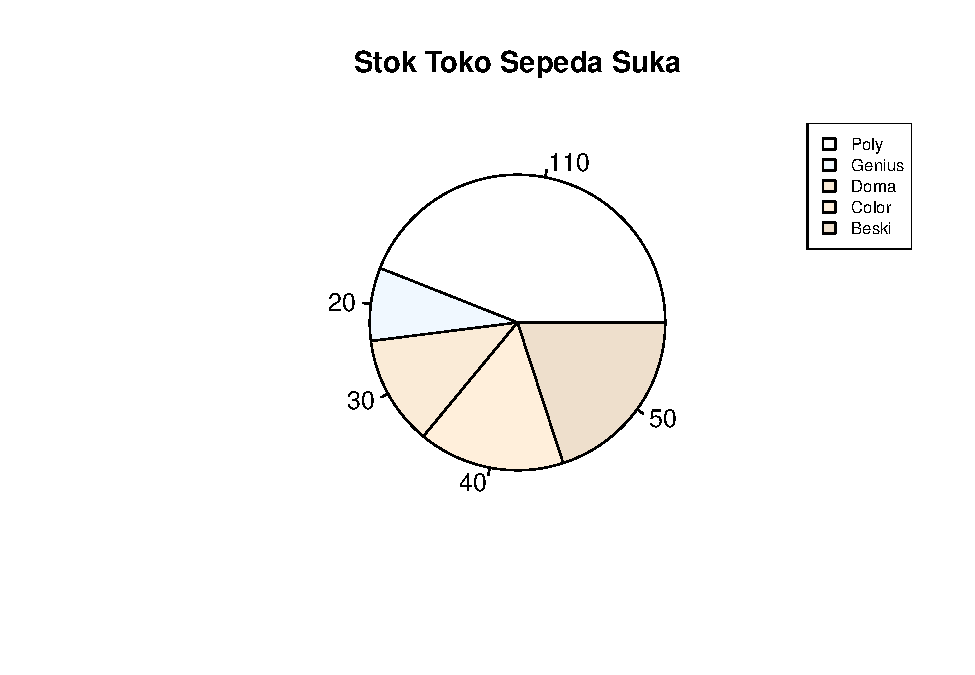
\includegraphics{_main_files/figure-latex/unnamed-chunk-13-2.pdf}

\hypertarget{grafik-daun-atau-steam-leaf}{%
\section{Grafik Daun atau Steam leaf}\label{grafik-daun-atau-steam-leaf}}

Grafik daun ini seperti bentuk pohon yang mmepunyai daun-daun. aadapun pohon terdiri yang cabang merupakan kategori dari yang kita cari. Pada data berkelompok atau mungkin data tidak berkelompok kita bisa membuatkan kelompok tersebut. Dengan grafik daun maka kita bisa menmapilkan data dalam kelompok. Batang tersebut adlah nilai yang menjdi kelas dalam distribusi frekuensi.
Yang menjdi daun adalah nilai-nilai angka. Bagi yang awalnya belum pernah membaca bentuk grafik ini mungkin akan membeinggungkan anda. Namum bukan berarati angka-angka yang ada tidak mempunyai arti yang berarti angka di belakang data tersebut.
jika membuat manual maka data-data ini akan sulit sebab kita harus menelsuri data-data yang menjadi anggota kelas tersebut.
Pemilihan Grafik Data
Setiap grafk mempunyai keistimewaaan dan kekurangan. Maka kita harus memakainya dengan bijak. Kalau grafik di BPS maka kemungkinan ada banyak yang akan menggunakan grafik berupa batang dan garis saja. Kedua grafik ini umum dan bisa menggambarkan data jenis apa saja. (Sukestiyarno, 2014)
Penggunaan grafik bantang mungkin kurang menarik daripada penggunaan grafik lingkaran namun penggunaan grafik ini akan membuat lebih efisien. Efisien dalam menyakian data yang sudah tersedia.

\begin{Shaded}
\begin{Highlighting}[]
\CommentTok{\#membuat vector data nilai kelas statistika}
\NormalTok{nilaistatistika }\OtherTok{=} \FunctionTok{c}\NormalTok{(}\DecValTok{78}\NormalTok{,}\DecValTok{45}\NormalTok{,}\DecValTok{67}\NormalTok{,}\DecValTok{76}\NormalTok{,}\DecValTok{55}\NormalTok{,}\DecValTok{68}\NormalTok{,}\DecValTok{59}\NormalTok{,}\DecValTok{42}\NormalTok{,}\DecValTok{74}\NormalTok{,}\DecValTok{64}\NormalTok{)}
\CommentTok{\#membuat perintah grafik daun }
\FunctionTok{stem}\NormalTok{(nilaistatistika)}
\end{Highlighting}
\end{Shaded}

\begin{verbatim}
## 
##   The decimal point is 1 digit(s) to the right of the |
## 
##   4 | 25
##   5 | 59
##   6 | 478
##   7 | 468
\end{verbatim}

Dapat kita lihat nilai tersebut adalah 4 nilai dari puluhan yang merupakan nilai dari stataistika sendagnkan 2 dan 5 adalah mewakili nilia 42 dan 45 dan seterusnya ke bawah

\hypertarget{latihan}{%
\section*{Latihan}\label{latihan}}
\addcontentsline{toc}{section}{Latihan}

\begin{enumerate}
\def\labelenumi{\arabic{enumi}.}
\tightlist
\item
  Apakah jenis grafik yang dapat digunakan untuk jenis data berkala? Jelaskan?
\item
  Jelaskan komponen dalam grafik daun? Apakah grafik ini efisien untuk data yang banyak jelaskan pendapat anda?
\item
  Buatlah grafik pie yang terdiri dari kategori berikut
  Anis 52\%
  Prabowo 25\%
  Ganjar 16\%
\item
  Cobalah interprestasikan grafik daun yang ada di sana. Sebutkan data-data yang ada dalam grafik daun tersebut?
\item
  Sebagai mahasiswa manajemen anda mendapatkan tugas untuk menyelidiki hal berikut:
\end{enumerate}

\begin{enumerate}
\def\labelenumi{\alph{enumi}.}
\tightlist
\item
  Harga saham yang meningkat ketika terjadinya perang Iran
\item
  Menurunnya pemasaran seblak pada tahun ini
\item
  Pekerja yang tetap kualitasnya meksi sudah mendapatkan uang honor tambahan
\item
  Google trend tentang suatu trend di website
\end{enumerate}

\hypertarget{ukuran-pemusatan}{%
\chapter{Ukuran Pemusatan}\label{ukuran-pemusatan}}

Kita membicarakan tinggi orang Indonesia lebih rendah daripada orang Eropa. Itu sudah menjadi suatu yang umum yang sudah ketahuai sebelumnya. Kita tidak asing dengan hal yang seperti itu karenanya sudah menjadikan suatu hal yang biasa. Pada saat out kita sudah berhasil untuk memberikan gambaran mengenai suatau kelompok dengan suatu kelompok yang lainnya.
Perbandingan tersebut mungkin akan memberikan suatau highlight kalau ada orang yang mau bertanya tentang suatu hal apa saja. Itu adalah satu bentuk pencirian atau deskripsi pada suatu hal atau obyek yang bisa manusia, mahluk hidup lainnya dan juga benda mati. Kalau kita memberikan suatu deskripsi yang Panjang mungkin itu lebih baik namun hal itu tidak sederhana dan mungkin bagi banyak orang hal itu tidak perlu namun dengan suatu pencirian yang cukup sederhana itu kita bisa untuk memberikan suatau hal yang berguna atau memberikan informasi yang berguna bagi masyarakat ataupun orang lain.
Ketika kita melihat suatu tabel ataupun grafik maka kita tidak semata untuk melihat tersebut dan hanya menuliskan beberapa kata apalagi cuma satu dua kalimat dalam menjelaskan tabel tersebut seolah-olah pembaca laporan harus melihat tabel tersebut sendiri padahal sebenarnya inilah kemampuan kita dalam membuat laporan tersebut bagaimana untuk menerangkan ini ada beberapa langkah-langkah yang dapat kita lakukan pertama tulislah jelas mengenai apa yang ada dalam grafik tersebut Langkah kedua kemudian memberikan informasi sebagai suatu rangkuman dalam tabel tersebut ini bisa banyak kemudian tulis tentang apa saja yang sangat signifikan dalam tabel tersebut langkah keempat menuliskan yang kurang signifikan atau yang di bawah signifikan yang paling signifikan kemudian langkah kelima dan membandingkan antara yang signifikan dengan tidak signifikan tersebut kemudian kita memberikan beberapa macam terakhir adalah informasi mengenai tabel tersebut
Dalam ukuran pemusatan berarati nilai-nilai data itu bersifat yang mendekati suatau titik. Tentu ini berbeda seperti misalnya disuatau tempat mempunyai jumlah konsumsi beras yang banyak akan tetapi di daerah tertentu mempunyai konumsi beras yang lebih sedikit karena adanya makanan pengganti beras seperti sagu. Tetapi dari satu data set tersebut akan bisa mempunyai karaterk rata-rata sendiri maupun ukran yang busa menjadi ``perwakilan'' dari kumpulan data tersebut. maka ada beberapa hal yang bisa kita lakukan dengan perhitungan dalam ukuran pemusatan tersebut seperti yang ada di bawah ini:
1. Rata-rata: rata rata adalah nilai keseluruhan jumlah data dibagi dengan jumlah data. Ini adalah ukuran pemusatan dan yang paling mudah untuk dicari angkanya dengan perhitungan tersebut. Nilai ini adalah merupakan perkiraaan dari nilai yang akn muncul dalam seluruh nilau atau jumlah data tersebut. Suatu rata-rata adalah mewakili daripada satu set atau sekelompok data. Karena rata-rata cenderung berada di tengah maka disebut juga sebagai ukuran pemusatan.
Rumus rata -rata arimetika adalah sebagai berikut

Rata-rata sebenarnya
\# Rata-rata Populasi dan Rata-rata Sampel

Rata-rata Populasi
Rumus rata-rata populasi, yang dilambangkan dengan \(\mu\), dapat dituliskan sebagai:

\[
\mu = \frac{\sum_{i=1}^{N} x_i}{N}
\]

\textbf{Keterangan:}
- \(x_i\) adalah nilai setiap elemen dalam populasi
- \(N\) adalah jumlah total elemen dalam populasi

Rata-rata Sampel
Rumus rata-rata sampel, yang dilambangkan dengan \(\bar{x}\), dapat dituliskan sebagai:

\[
\bar{x} = \frac{\sum_{i=1}^{n} x_i}{n}
\]

\textbf{Keterangan:}
- \(x_i\) adalah nilai setiap elemen dalam sampel
- \(n\) adalah jumlah total elemen dalam sampel
Dalam rata-rata tersebut ada huruf aksara Yunani (Greek Alphabet). Yang dibaca MU untuk nilai ini berarti adalah rata-rata dari rata sebanrnya atau disebut juga rata-rata populasi. Sedangkan ada rata-ata perkiraaan karena menggunakan nilai
Apakah itu rata-rata sebenarnya dan perkiraan?
Rata-rata sebenarnya itu adalah menghitung suatu rata-rata dalam populasi. Kalau kita menghitung perkiraaan maka kita menghitung rata-rata dari nilai yang dihitung dari sample.\\
Kalau masalah sample itu sekarang kita bisa memilih ada yang populasi tidak terbatas atau infinite maka kita akan sulit untuk menentukan jumlah populasi. Seperti kalau populasi mahasiswa di universitas tertentu. Sepanjang kalau kita tidak memenutukan populasi maka kita tidak akan bisa untuk menentukan sample yang hendak kita gunakan.

\begin{enumerate}
\def\labelenumi{\arabic{enumi}.}
\setcounter{enumi}{1}
\tightlist
\item
  Rata-rata Geomettri
  Rata-rata geomteri adalah nilai rata-rata beberapa angka yang sudah disediakan. kita membuat suatu angka tersebut yang dari rata-rata. Dalam menghitung tersebut kita bukan lagi menambahkan seperti rata-rata aritmetik karena nilai tersebut sudah berbeda. Dalam rata-rata geometri maka kita akan mengalikan dengan nilai yang ada dan kemudian membuat akar dari perkalian tersebut.
\end{enumerate}

Rata-rata geometri untuk sekumpulan data \(x_1, x_2, \dots, x_n\) dapat dihitung dengan rumus berikut:

\[
\text{Geometric Mean} = \sqrt[n]{x_1 \cdot x_2 \cdot \dots \cdot x_n} = \left( \prod_{i=1}^{n} x_i \right)^{\frac{1}{n}}
\]

\textbf{Keterangan:}
- \(x_i\): Nilai setiap elemen dalam sekumpulan data.
- \(n\): Jumlah elemen dalam sekumpulan data.
- \(\prod\): Notasi untuk perkalian berurutan dari semua elemen \(x_i\) dari \(i = 1\) hingga \(n\).

Rata-rata geometri biasanya digunakan ketika data memiliki sifat perkalian atau mengalami pertumbuhan berkelanjutan, seperti dalam data ekonomi atau pengembalian investasi.

Rata-rata geometri tentu berbeda dengan cara seperti mengalikan keseluruhan nilai yang ada, seperti pada kasus kecepatan. Kecepatan itu tentu berlaku pada jarak yang berbeda seperti antara kecepatan 50 km/jam atau 100 km/jam mungkin keduanya mengalami jarak tempuh yang berbeda yang tidak dapat di rata-ratakan secara aritmetika maka tidak bisa dilakukan dengan cara itu.

\begin{enumerate}
\def\labelenumi{\arabic{enumi}.}
\setcounter{enumi}{2}
\tightlist
\item
  Rata-Rata Harmoni
  Rata-rata Harmoni adalah rata-rata yang membagi jumlah nilai dengan nilai data yang merupakan kebalikan.
\end{enumerate}

Rata-rata harmonik untuk sekumpulan data \(x_1, x_2, \dots, x_n\) dapat dihitung dengan rumus berikut:

\[
\text{Harmonic Mean} = \frac{n}{\sum_{i=1}^{n} \frac{1}{x_i}}
\]

\textbf{Keterangan:}
- \(x_i\): Nilai setiap elemen dalam sekumpulan data.
- \(n\): Jumlah elemen dalam sekumpulan data.
- \(\sum\): Notasi untuk penjumlahan dari \(i = 1\) hingga \(n\).

Rata-rata harmonik sering digunakan dalam situasi di mana kecepatan, rasio, atau tingkat perubahan lebih relevan, seperti dalam perhitungan kecepatan rata-rata atau analisis data keuangan.

\begin{enumerate}
\def\labelenumi{\arabic{enumi}.}
\setcounter{enumi}{3}
\tightlist
\item
  Median: Ini adalah nilai tengah dari kumpulan satu set data ini mengambarkan nilai yang berada di tengah. Kalau nilai tengah ini tentu berbeda karena cara menghitungnya adalah berbeda. Tidak ada rumus untuk menghitung untuk data yang Pada median maka kita menyusun data yang rendah sampai yang tertinggi adalah dengan cara mengurutkan dan kita mendapatkan nilai yang tengha. kalau ada nilai yang ada di tengah maka itulah itu nilai median. Maka untuk nilai tengah ini kita tidak bisa membuat sama. Terkadang pada beberapa kausus
  Median tidak mempunyai rumus untuk data yang tidak berkelompok. Untuk median kita membaginya dengan data yang berada di urutan yang di tengah. Kalau data tersebut berjumlah ganjil maka itu yang berada yang ada di tengah sedangkan kalau nilainya adalah genap maka data yang menjadi median adalah yang berada di tengah namun karena genap itu tidak ada yang pas di tengah dan ada yang dua di tengah maka kita pilih rata-rata dari dua bilangan yang berturut misalnya kalau untuk bilangan berjumlah enam maka kita bagi menjadi tiga-tiga maka letak dari nilai tersebut itu adalah nilai dari median tersebut.
\end{enumerate}

Rumus Median untuk data berjumlah ganjil adalah Me= data ke (n+1)/2
Rumus Median untuk data berjumlah ganjil adalah Me= data ke {[}data ke(n:2)+data ke (:2) +1{]}/2

\begin{enumerate}
\def\labelenumi{\arabic{enumi}.}
\setcounter{enumi}{4}
\tightlist
\item
  Modus adalah ukuran yang menunjukkan suatu data yang sering muncul dalam satu set data. Terkadang ada juga muncul modus yang lebih dari satu. Untuk mencari data modus data yang tidak berkelompok ini kita perlu juga mengurutkan bilangan tersebut. Setelah mengurutkan nilai tersebut kita akan melihat nilai-nilai dari yang sudah disusun tersebut Kita memilih beberapa dari nilai yang tersebut. Maka dengan demikian kita sudah mendapatkan modus. Dengan melihat banyaknya modus kita bisa mamperkirakan sebaran data yang paling banyak muncul. Kalau dalam suatu perkara maka si penyelidik atau detektif akan melihat mana yang terus menerus menjadi modus.
  Dalam modus kita bisa menginterprestasikan bahwa data yang sering muncul adalah sejumlah tertentu. Dengan adanya modus kita bisa melihat bahwa data yang sering muncul adalah data tersebut.
\end{enumerate}

Sifat-sifat modus adalah
Kelebihan dan kekurangan modus
Interprestasi modus

Latihan
Apa kegunaan mean dalam statistik deskriptif?
Bagaiamana median di hitung dan apa peranannya dalam ukuran pemusatan?
Jelaskan konsep modus dan apa signifikansinya dalam statistik deskriptif?
Pada saat situasi apa nilai rata-rata atau mean lebih menggambarkan daripada median?
Definisikan rata-rata tertimbang dan bagaiamana penggunaan dalam statistik
Bagaimana pilihan dari statistik atau baik mode, mean, median dalam menggambarkan atau mendeskripsikan dari ukuran pemusatan atau cenral tendency
Gambarkan perhitungan rata-rata geometri dan praktikal dan aplikasinya?
Diskusi tentang rata-rata harmoni dan aplikasinya?
Perbandingan mean, modus , and median?

Glossary
Mean
Median
Modus
Rata-rata Geometri
Rata-rata Harmoni

\hypertarget{ukuran-penyebaran}{%
\chapter{Ukuran Penyebaran}\label{ukuran-penyebaran}}

Setelah kita mengetahui namanya ukuran pemusatan maka kita akan mempelajari ukuran penyebaran tersebut atau ukuran variasi kita menyadari bahwa dalam satu kelompok sampel data maka kita akan tahu tidak semuanya sama bahkan seorang pegawai dengan kemampuan sama pengalaman sama dan tanggungan yang sama gajinya tidak sama persis itu yang terjadi di perusahaan maka kita juga harus tahu bahwa tidak semua ada data yang terdistribusi tidak normal ada satu kecenderungan di negara-negara maju orang lebih jauh sejahtera sedangkan yang miskinnya dikit sedangkan negara-negara terbelakang hanya sedikit orang yang kaya dan orang yang miskin banyak sekali. Pada gambar tetapi secara keseluruhan data memang kita akui bahwa negara-negara ketiga tidak ada yang kekayaannya melebihi orang-orang di negara maju walaupun memang seperti di negara kita ada negara ada pengusaha yang super kaya tetapi kalau dibandingkan dengan pengusaha di Amerika seperti emas tentu tidak setara seperti itu nah karena rata-rata tersebut saya masih bisa gunakan untuk menggambarkan salah satu populasi ataupun dari sampel tersebut tetapi pada kenyataannya bahwa ada beberapa kelompok tertentu yang rata-ratanya sama itu ternyata banyak yang tidak lulus misalnya di kelas A dan plastik tersebut mempunyai rata-rata yang sama 60 tetapi di kelas A itu ternyata tidak banyak yang lulus Hal ini karena di kelas aa aja ada nilai yang sangat tinggi sekali sedangkan ada yang nilai kebanyakan rendah sekali jadi nilai-nilai yang tinggi tersebut menutupi nilai-nilai rendah tetapi sebagai syarat kelulusan dari mahasiswa kelas A tidak memenuhi sehingga banyak dari mahasiswa yang di sini daerah rata-ratanya lebih tinggi Maka itu banyak yang tidak lulus nah karena itu kenapa kita mempelajari ukuran penyebaran karena kadang-kadang di beberapa kasus memang tidak berlaku sepenuhnya rata-rata yang sudah tersebut.
Tentu seperti diuraikan di atas banyak faedah daripada kita mempelajari ukuran penyebaran tersebut kita di dalam dunia investasi mengenal apa yang namanya risiko sebagai bentuk dari konsekuensi daripada keuntungan yang diharapkan jadi kalau keuntungan itu bisa saja tinggi tetapi juga bisa jadi akan rendah ketika atau manakala suatu resikonya besar sekali dan dalam dunia investasi kita mengenal bahwa tingginya resiko akan setara dengan tingginya keuntungan yang diharapkan

Beberpa ahli stataistik mencoba untuk mengukur beberapa data yang menyebar. adapun ukuran data yang digunakan untuk penyebaran data adalah sebagai berikut

\hypertarget{ukuran-variansi}{%
\section*{1. Ukuran Variansi}\label{ukuran-variansi}}
\addcontentsline{toc}{section}{1. Ukuran Variansi}

Ukuran ini yang sering digunakan dengan merupakan jumlah selisjih kuadrat dari tiap bilangan dengan rata-rata diagi dengan jumlah set data. Tentu tidak semua bilanhan akanbsama dengan rata-rata. Kalau ada sermua seragam seperti terjadinya nilai ujian yang sama oerssi mislanya ujian dengan bentuk soal pilihan ganda yang akan menghasilkan nilai yang sama maka
Sample Variance
s\^{}2=(∑▒(x-x ̅ )\^{}2 )/(n-1)
Dimana
S2 : Simpangan Variance
x : Nilai x
x ̅ : Rata-rata X
n : banyaknya data

\[
s^2 = \sqrt{\frac{1}{n - 1} \sum_{i=1}^{n} (x_i - \bar{x})^2}
\]

\textbf{Keterangan:}
- \(x_i\): Nilai setiap elemen dalam sampel.
- \(\bar{x}\): Rata-rata sampel.
- \(n\): Jumlah elemen dalam sampel.
- \((n - 1)\): Penyebut ini digunakan dalam sampel untuk menghasilkan estimasi tak bias dari standar deviasi populasi.
- \((x_i - \bar{x})^2\): Kuadrat dari deviasi setiap elemen terhadap rata-rata sampel.

\begin{enumerate}
\def\labelenumi{\arabic{enumi}.}
\setcounter{enumi}{1}
\tightlist
\item
  Ada simpangan rata-rata yang merupakan selisih antara tiap nilai dengan nilai rata-ratanya tersebut. Jadi tiap nilai dikurangi dengan nilai rata-ratanya dalam bentuk nilai yang absolut atau tidak bisa negatif setelah itu baru kita bagikan dari jumlah nilai selisih yang absolut tersebut dengan jumlah nilai yang kita gunakan.. Rumusnya adalah sebagai berikut:
\end{enumerate}

Simpangan rata-rata adalah ukuran dispersi yang menunjukkan rata-rata dari nilai absolut deviasi setiap data terhadap rata-rata. Rumus simpangan rata-rata untuk data \(x_1, x_2, \dots, x_n\) adalah sebagai berikut:

\[
\text{Simpangan Rata-rata} = \frac{1}{n} \sum_{i=1}^{n} |x_i - \bar{x}|
\]

\textbf{Keterangan:}
- \(x_i\): Nilai setiap elemen dalam data.
- \(\bar{x}\): Rata-rata dari seluruh data.
- \(n\): Jumlah elemen dalam data.
- \(\sum\): Notasi penjumlahan dari \(i = 1\) hingga \(n\).
- \(|x_i - \bar{x}|\): Nilai absolut dari selisih antara \(x_i\) dan rata-rata \(\bar{x}\), yang menunjukkan deviasi setiap data terhadap rata-rata.

Simpangan rata-rata memberikan informasi tentang seberapa jauh rata-rata setiap data dari rata-rata keseluruhan.

\hypertarget{ukuran-standar-deviasi}{%
\section*{2 ukuran standar deviasi}\label{ukuran-standar-deviasi}}
\addcontentsline{toc}{section}{2 ukuran standar deviasi}

Ini adalah ukuran penyebaran yang lebih mudah difahami oleh penguna stataistik. Kita akan melihat standar deviasi atau standar simpangan yang ada dengan cara melihat dari nilai ini atau dari deviasi adalah atau merupakan akar kuadrat dari variansi
Nilai akar kuadrat uang lebih kecil daripada variansi memberikan suatau ukuran yang lebih diterima oleh pembaca atau pengguna data yang masih belum mengetahui nilai statistik.
Jika kita memiliki data populasi \(x_1, x_2, \dots, x_N\), standar deviasi populasi (\(\sigma\)) dihitung dengan rumus:

\[
\sigma = \sqrt{\frac{1}{N} \sum_{i=1}^{N} (x_i - \mu)^2}
\]

\textbf{Keterangan:}
- \(x_i\): Nilai setiap elemen dalam populasi.
- \(\mu\): Rata-rata populasi.
- \(N\): Jumlah elemen dalam populasi.
- \(\sum\): Notasi penjumlahan dari \(i = 1\) hingga \(N\).
- \((x_i - \mu)^2\): Kuadrat dari deviasi setiap elemen terhadap rata-rata populasi.

Standar Deviasi Sampel
Jika kita memiliki data sampel \(x_1, x_2, \dots, x_n\), standar deviasi sampel (\(s\)) dihitung dengan rumus:

\[
s = \sqrt{\frac{1}{n - 1} \sum_{i=1}^{n} (x_i - \bar{x})^2}
\]

\textbf{Keterangan:}
- \(x_i\): Nilai setiap elemen dalam sampel.
- \(\bar{x}\): Rata-rata sampel.
- \(n\): Jumlah elemen dalam sampel.
- \((n - 1)\): Penyebut ini digunakan dalam sampel untuk menghasilkan estimasi tak bias dari standar deviasi populasi.
- \((x_i - \bar{x})^2\): Kuadrat dari deviasi setiap elemen terhadap rata-rata sampel.

Standar deviasi menggambarkan seberapa jauh rata-rata penyebaran data dalam sekumpulan data, baik itu populasi atau sampel.

\hypertarget{rentang}{%
\section*{3. Rentang}\label{rentang}}
\addcontentsline{toc}{section}{3. Rentang}

Rentang atau Range juga bisa menjadi suatu ukuran penyebaran data karena dari rentang ini kita akan melihat seberapa besar nilai rentang antara yang terbesar dan yang terkecil contoh lalu nilai maksimum yaitu bisa 10 kali dari nilai minimum ya maka akan menghasilkan rentang yang besar sekali atau terjadinya suatu varian yang besar sekali dari tentang sendiri sebenarnya sudah bisa diduga sebuah set data atau kumpulan data sampel itu bisa menunjukkan apa Data tersebut mempunyai varian sebesar.

\hypertarget{sifat-dari-varians}{%
\section*{4. Sifat dari varians}\label{sifat-dari-varians}}
\addcontentsline{toc}{section}{4. Sifat dari varians}

Kita perlu mempelajari bahwa salah satu bentuk ukuran adalah ukuran penyebaran adalah panjang adalah variasi ya jadi memang tidak ada di dunia ini Maka ada beberapa sifat yang bisa kita ketahui dari variasi tersebut: garis baru
1. Varians mempunyai perhitungan atau nilai yang selalu positif Karena perhitungan selisih dari tiap angka tersebut dengan rata-rata sudah positif karenanya delay khasiat akan selalu positif kamu ganti baju
2. Karena nilai tersebut positif maka ada yang menilai besar dan juga nilai yang kecil nilai besar itu disebabkan karena selisih dari nilai individu dengan nilai rata-rata itu besar sekali makanannya ada simpan nilai jenis variasi nya besar sekali aku berada sebaliknya dengan nilai variasi yang kecil maka akan menunjukkan bahwa data tersebut mempunyai variasi yang rendah atau perbedaan antara beberapa data yang masuk dalam set anggota tersebut tidak beberapa besar itu baris baru baris baru
3. Karena nilai ini adalah variasi maka nilai varians akan sensitif terhadap nilai-nilai yang outlier atau nilai-nilai yang sangat jauh berbeda dengan ukuran pemusatannya begitu ada nilai out layernya yang masuk maka dapat dipastikan nilai variansnya akan berbeda dan akan menunjukkan suatu nilai yang lebih tinggi daripada nilai sebelumnya.
4. Tentu banyaknya itu akan bisa diatasi misalnya dengan peng-kuadratkan nilai atau dengan melakukan logaritma hingga membuat data-data tersebut menjadi lebih seragam nah ini berapa teknik ini dilakukan untuk memuluskan suatu asumsi model..

\hypertarget{soal-latihan-ukuran-penyebaran}{%
\section*{Soal Latihan Ukuran Penyebaran}\label{soal-latihan-ukuran-penyebaran}}
\addcontentsline{toc}{section}{Soal Latihan Ukuran Penyebaran}

1 Pak Samin mengadakan ujian matematika dan dari 10 siswa itu diperoleh data nilai mahasiswa di kelas A1 adalah sebagai berikut:

70, 80, 90, 100, 110, 120, 130, 140, 150, 160

Hitunglah:

\begin{itemize}
\tightlist
\item
  Jangkauan
\item
  Simpangan rata-rata
\item
  Simpangan baku
\end{itemize}

\begin{enumerate}
\def\labelenumi{\arabic{enumi}.}
\setcounter{enumi}{1}
\tightlist
\item
  PT Asti ingin mengetahui profil dari variasi gaji karyawannya sebanyak 10 orang:
\end{enumerate}

Rp 2.000.000, Rp 3.500.000, Rp 4.000.000, Rp 5.000.000, Rp 6.000.000, Rp 7.000.000, Rp 8.000.000, Rp 9.000.000, Rp 9.500.000

Hitunglah:

\begin{itemize}
\tightlist
\item
  Kuartil pertama
\item
  Kuartil ketiga
\item
  Simpangan kuartil
\end{itemize}

\begin{enumerate}
\def\labelenumi{\arabic{enumi}.}
\setcounter{enumi}{2}
\tightlist
\item
  toko emas intan berlian ingin mengetahui profil dari penjualannya hari ke hari. Ia mencatat beberapa penjualan selama 10 hari dan ingin mengetahui variasi yang terjadi
\end{enumerate}

17, 12, 15, 18, 20, 22, 23, 28, 30, 32

Hitunglah:

\begin{itemize}
\tightlist
\item
  Median
\item
  MAD
\item
  Skewness
\end{itemize}

\begin{enumerate}
\def\labelenumi{\arabic{enumi}.}
\setcounter{enumi}{3}
\tightlist
\item
  Dalam setiap produksi PT Baja selalu mengukur standar tetapi hasil yang diberikan oleh para suppliernya berbeda-beda makanannya PT Baja ingin mengetahui setidaknya dari 20 sampel variasi dari produk barang tersebut:
\end{enumerate}

101, 101, 102, 103, 104, 105, 106, 107, 108, 109, 110, 111, 111, 112, 114, 115, 116, 117, 118, 119

Hitunglah:

\begin{itemize}
\tightlist
\item
  Jangkauan
\item
  Simpangan rata-rata
\item
  Simpangan baku
\item
  Kurtosis
\end{itemize}

\begin{enumerate}
\def\labelenumi{\arabic{enumi}.}
\setcounter{enumi}{4}
\tightlist
\item
  t PT kontraktor selalu jaya ingin mengetahui berapa lama penyelesaian suatu proyek karena ada beberapa proyek yang dilakukan dalam waktu singkat dan juga elektrolit digunakan dalam waktu tertentu
\end{enumerate}

\begin{verbatim}
10 hari, 12 hari, 15 hari, 18 hari, 20 hari, 22 hari, 25 hari, 28 hari, 30 hari, 32 hari
\end{verbatim}

Hitunglah:

\begin{itemize}
\tightlist
\item
  Jangkauan
\item
  Simpangan rata-rata
\item
  Simpangan baku
\item
  Skewness
\item
  Kurtosis
\end{itemize}

Bonus:

Jelaskan secara singkat perbedaan antara simpangan rata-rata dan simpangan baku.

\hypertarget{statistik-deskriptif-dengan-rsstudio}{%
\chapter{Statistik Deskriptif dengan RSstudio}\label{statistik-deskriptif-dengan-rsstudio}}

Seperti kita ketahui R Studio juga bisa untuk menghitung statistik deskrptif dengan ukuran pemusatan maupun ukuran penyebaran. Kita bisa menggunakan untuk data-data seperti vector, data frame, atau lainnya ada beberapa fungsi yang bisa kita lakukan kita mulai dengan vector

Vector sudah kita bahasa adalah sebuah data dan kita akang menggunakan vector untuk deskriptif statistik. Penulis akan gunakan vektor sebelumnya yakni nilai statistika. kita menggunakan fungsi pertama adalah summary

\begin{Shaded}
\begin{Highlighting}[]
\FunctionTok{summary}\NormalTok{(nilaistatistika)}
\end{Highlighting}
\end{Shaded}

\begin{verbatim}
##    Min. 1st Qu.  Median    Mean 3rd Qu.    Max. 
##    42.0    56.0    65.5    62.8    72.5    78.0
\end{verbatim}

\begin{Shaded}
\begin{Highlighting}[]
\FunctionTok{sd}\NormalTok{(nilaistatistika)}
\end{Highlighting}
\end{Shaded}

\begin{verbatim}
## [1] 12.47932
\end{verbatim}

Pada bagian perintah ini kita bisa melihat ada beberapa nilai MIn artinya nilai yang paling kecil atau minimal maximal nilai yang paling besar. Dalam fungsi ini tidak ada standar deviasi ataupun varians. kita bsia mengetik dengan perintah sd atau singnkatan dari stndard deviasi. KIta bis alihat di artikel ini \citet{Platter2024}

Perintah untuk menghitung statsitik deskriptif kita bisa lakukan pada data. frame dengan mengetik perintah yang sama yakni summary seperti dibawah ini menggunakan data.frame dat.coba.

\begin{Shaded}
\begin{Highlighting}[]
\FunctionTok{summary}\NormalTok{(datcoba)}
\end{Highlighting}
\end{Shaded}

\begin{verbatim}
##       id                saving          income    
##  Length:7           Min.   :100.0   Min.   :1000  
##  Class :character   1st Qu.:125.0   1st Qu.:1125  
##  Mode  :character   Median :150.0   Median :1200  
##                     Mean   :164.3   Mean   :1214  
##                     3rd Qu.:200.0   3rd Qu.:1275  
##                     Max.   :250.0   Max.   :1500
\end{verbatim}

Kita lihat bahwa masing-masing kolom dari tabel mempunyai nilai minimal (Min), kuartil pertama (1st Qu), Median atau Nilai Tengah (Median), rata-rata (mean), kuartil ketiga (3rd Qu), dan Max atau nilai tertinggi. Hanya saja tidak ada standard deviasi. penggunaan perintah sd pada data. frame tidak bisa dilakukan.

\hypertarget{footnotes-and-citations}{%
\chapter{Footnotes and citations}\label{footnotes-and-citations}}

\hypertarget{footnotes}{%
\section{Footnotes}\label{footnotes}}

Footnotes are put inside the square brackets after a caret \texttt{\^{}{[}{]}}. Like this one \footnote{This is a footnote.}.

\hypertarget{citations}{%
\section{Citations}\label{citations}}

Reference items in your bibliography file(s) using \texttt{@key}.

For example, we are using the \textbf{bookdown} package \citep{R-bookdown} (check out the last code chunk in index.Rmd to see how this citation key was added) in this sample book, which was built on top of R Markdown and \textbf{knitr} \citep{xie2015} (this citation was added manually in an external file book.bib).
Note that the \texttt{.bib} files need to be listed in the index.Rmd with the YAML \texttt{bibliography} key.

The RStudio Visual Markdown Editor can also make it easier to insert citations: \url{https://rstudio.github.io/visual-markdown-editing/\#/citations}

\hypertarget{blocks}{%
\chapter{Blocks}\label{blocks}}

\hypertarget{equations}{%
\section{Equations}\label{equations}}

Here is an equation.

\begin{equation} 
  f\left(k\right) = \binom{n}{k} p^k\left(1-p\right)^{n-k}
  \label{eq:binom}
\end{equation}

You may refer to using \texttt{\textbackslash{}@ref(eq:binom)}, like see Equation \eqref{eq:binom}.

\hypertarget{theorems-and-proofs}{%
\section{Theorems and proofs}\label{theorems-and-proofs}}

Labeled theorems can be referenced in text using \texttt{\textbackslash{}@ref(thm:tri)}, for example, check out this smart theorem \ref{thm:tri}.

\begin{theorem}
\protect\hypertarget{thm:tri}{}\label{thm:tri}For a right triangle, if \(c\) denotes the \emph{length} of the hypotenuse
and \(a\) and \(b\) denote the lengths of the \textbf{other} two sides, we have
\[a^2 + b^2 = c^2\]
\end{theorem}

Read more here \url{https://bookdown.org/yihui/bookdown/markdown-extensions-by-bookdown.html}.

\hypertarget{callout-blocks}{%
\section{Callout blocks}\label{callout-blocks}}

The R Markdown Cookbook provides more help on how to use custom blocks to design your own callouts: \url{https://bookdown.org/yihui/rmarkdown-cookbook/custom-blocks.html}

\hypertarget{sharing-your-book}{%
\chapter{Sharing your book}\label{sharing-your-book}}

\hypertarget{publishing}{%
\section{Publishing}\label{publishing}}

HTML books can be published online, see: \url{https://bookdown.org/yihui/bookdown/publishing.html}

\hypertarget{pages}{%
\section{404 pages}\label{pages}}

By default, users will be directed to a 404 page if they try to access a webpage that cannot be found. If you'd like to customize your 404 page instead of using the default, you may add either a \texttt{\_404.Rmd} or \texttt{\_404.md} file to your project root and use code and/or Markdown syntax.

\hypertarget{metadata-for-sharing}{%
\section{Metadata for sharing}\label{metadata-for-sharing}}

Bookdown HTML books will provide HTML metadata for social sharing on platforms like Twitter, Facebook, and LinkedIn, using information you provide in the \texttt{index.Rmd} YAML. To setup, set the \texttt{url} for your book and the path to your \texttt{cover-image} file. Your book's \texttt{title} and \texttt{description} are also used.

This \texttt{gitbook} uses the same social sharing data across all chapters in your book- all links shared will look the same.

Specify your book's source repository on GitHub using the \texttt{edit} key under the configuration options in the \texttt{\_output.yml} file, which allows users to suggest an edit by linking to a chapter's source file.

Read more about the features of this output format here:

\url{https://pkgs.rstudio.com/bookdown/reference/gitbook.html}

Or use:

\begin{Shaded}
\begin{Highlighting}[]
\NormalTok{?bookdown}\SpecialCharTok{::}\NormalTok{gitbook}
\end{Highlighting}
\end{Shaded}


  \bibliography{book.bib,packages.bib}

\end{document}
